\documentclass[10pt]{article}

% Pacotes extras necessários
\usepackage{amsmath}
\usepackage[lmargin=0.5in, rmargin=0.5in, tmargin=0.5in, bmargin=0.5in, includehead, includefoot]{geometry}
\usepackage{amsfonts}
\usepackage[utf8]{inputenc}
\usepackage[portuguese]{babel}
\usepackage{graphicx}
\usepackage{fancyhdr}
\usepackage{setspace}
\usepackage{listings}
\usepackage{url}
\usepackage{enumitem}
\usepackage{appendix}
\usepackage{subcaption}
\usepackage[dvipsnames]{xcolor}
\usepackage{tikz}
\usetikzlibrary{positioning}

% Define estilo para listagens de código
\lstdefinestyle{mystyle}{
    language=Matlab,
    inputencoding=latin1,
    extendedchars=true,
    backgroundcolor=\color{white},
    basicstyle=\ttfamily\footnotesize,
    numbers=left,
    numberstyle=\tiny\color{gray},
    numbersep=5pt,
    tabsize=2,
    breaklines=true,
    keywordstyle=\color{blue},
    commentstyle=\color{green!60!black},
    stringstyle=\color{orange},
    frame=single,
    keepspaces=true,
    showspaces=false,
    showstringspaces=false,
    showtabs=false,
}
\lstset{style=mystyle}

\graphicspath{{./images/}}

\setlength{\parindent}{0pt}
\setstretch{1.5}

\DeclareMathOperator{\sen}{sen}
\DeclareMathOperator{\sinc}{sinc}
\newcommand{\Lap}[1]{\mathcal{L}\left\{#1\right\}}
\newcommand{\bm}[1]{\boldsymbol{#1}}

% Cabeçalho e rodapé em todas as páginas
\pagestyle{fancy}
\fancyhf{}
\fancyhead[L]{Relatório das simulações}
\fancyfoot[C]{\thepage}

% Dados do Grupo
\title{
    Trabalho Nº1 - MRAC Direto \\
    \large COE603 - Controle Adaptativo
}
\author{
    Caio Cesar Leal Verissimo - 119046624 \\
    Leonardo Soares da Costa Tanaka - 121067652 \\
    Lincoln Rodrigues Proença - 121076407 \\
    Engenharia de Controle e Automação - UFRJ \\
    Rio de Janeiro, Rio de Janeiro, Brasil \\
    Maio de 2025
}
\date{}

\begin{document}

\maketitle

% Geração automática do sumário
\tableofcontents
\newpage

\section{Resumo das equações do sistema}

Neste experimento, simulamos o algoritmo \textbf{MRAC Direto} para o caso:
\begin{itemize}
    \item $n = 1$ \hfill (ordem da planta)
    \item $n^* = 1$ \hfill (grau relativo)
    \item $n_p = 2$ \hfill (número de parâmetros)
\end{itemize}

\subsection{Equações do Algoritmo MRAC Direto}

A Tabela \ref{tab:equacoes_mrac} resume as equações fundamentais do algoritmo MRAC (Model Reference Adaptive Control) na forma direta, considerando uma planta de primeira ordem ($n = 1$), grau relativo igual a 1 ($n^* = 1$) e número de parâmetros $n_p = 2$.

\begin{table}[h!]
\centering
\begin{tabular}{|l|l|c|}
\hline
\textbf{Descrição}      & \textbf{Equação}                                  & \textbf{Ordem} \\ \hline
Planta                  & $\dot{y} = a_p y + k_p u$                         & 1              \\ \hline
Modelo                  & $\dot{y}_m = -a_m y_m + k_m r$                    & 1              \\ \hline
Erro da saída           & $e_0 = y - y_m$                                   &                \\ \hline
Lei de controle         & $u = \theta^T \omega$                  &                \\ \hline
Regressor               & $\omega^T = \begin{bmatrix} y & r \end{bmatrix}$ &                \\ \hline
Lei de adaptação        & $\dot{\theta} = -\text{sign}(k_p)\Gamma \omega e_0$ & 2 \\ \hline
\end{tabular}
\caption{Resumo do Algoritmo MRAC Direto}
\label{tab:equacoes_mrac}
\end{table}

A Figura \ref{fig:bloco_verificacao} ilustra o diagrama de blocos do sistema em malha fechada, juntamente com a verificação da equivalência com o modelo de referência. Este diagrama mostra como a combinação dos ganhos adaptativos $\theta_1^*$ e $\theta_2^*$ pode transformar o comportamento da planta para que ela imite o modelo de referência.

\begin{figure}[h!]
    \centering
    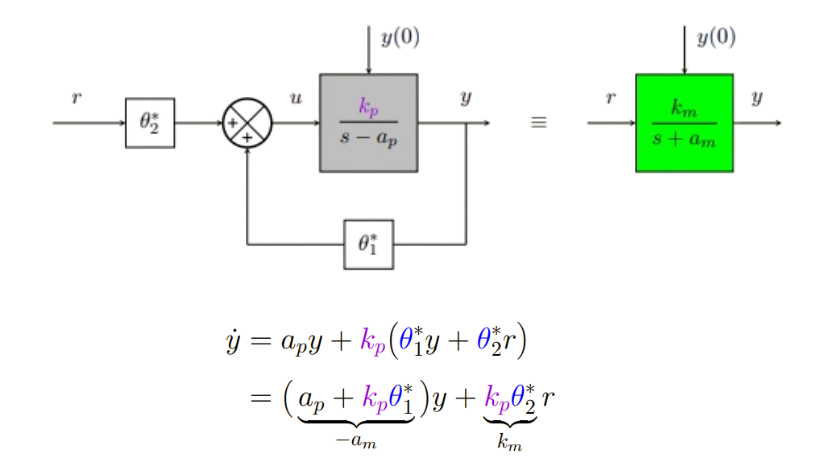
\includegraphics[width=0.6\textwidth]{img/diagrama.png}
    \caption{Diagrama de blocos e verificação da equivalência com o modelo de referência}
    \label{fig:bloco_verificacao}
\end{figure}

As expressões ideais para os parâmetros $\theta_1^*$ e $\theta_2^*$ que garantem essa equivalência são apresentadas a seguir. Esses parâmetros são obtidos por identificação direta, com base nas constantes do modelo e da planta.

\begin{center}
\begin{minipage}{0.3\textwidth}
\begin{center}
\fbox{
    $\theta_1^* = -\dfrac{a_p + a_m}{k_p}$
}
\end{center}
\end{minipage}
\begin{minipage}{0.3\textwidth}
\begin{center}
\fbox{
    $\theta_2^* = \dfrac{k_m}{k_p}$
}
\end{center}
\end{minipage}
\end{center}

Essas equações representam os valores ideais dos parâmetros adaptativos para que a planta controlada siga o comportamento especificado pelo modelo de referência. Na prática, o algoritmo de adaptação busca aproximar esses valores ao longo do tempo.

\subsection{Estabilidade do Algoritmo MRAC Direto}

\paragraph{1. Forma vetorial e definições}
Escrevendo em forma vetorial:
\begin{equation}
  \bm{\theta}^* = 
  \begin{bmatrix}
    \theta_1^* \\ \theta_2^*
  \end{bmatrix},
  \quad
  \bm{\omega} = 
  \begin{bmatrix}
    y \\ r
  \end{bmatrix}
  \quad\Longrightarrow\quad
  u^* = \bm{\theta}^{*T}\,\bm{\omega}.
\end{equation}
Analogamente, a lei de controle é
\begin{equation}
  \bm{\theta} = 
  \begin{bmatrix}
    \theta_1 \\ \theta_2
  \end{bmatrix}
  \quad\Longrightarrow\quad
  u = \bm{\theta}^T\,\bm{\omega}.
\end{equation}

\paragraph{2. Dinâmica do erro}
Definimos o erro de saída:
\begin{equation}
  e = y - y_m.
\end{equation}
Subtraindo as dinâmicas da planta e do modelo:
\begin{equation}
  \begin{aligned}
  \dot e 
  &= \dot y - \dot y_m
   = (a_p y + k_p u) - (-a_m y_m + k_m r) \\
  &= -a_m (y - y_m) + (a_p + a_m) y + k_p u - k_m r
    + \underbrace{(a_m y) - (a_m y)}_{=0} \\
  &= -a_m e
    + k_p\Bigl[\tfrac{a_p + a_m}{k_p}\,y + u - \tfrac{k_m}{k_p}\,r\Bigr] \\
  &= -a_m e + k_p \bigl[u - \theta_1^* y - \theta_2^* r\bigr] \\
  &= -a_m e + k_p \bigl[u - u^*\bigr].
  \end{aligned}
\end{equation}

\paragraph{3. Erro paramétrico}
Definimos o vetor de erro de parâmetro:
\begin{equation}
  \tilde{\bm{\theta}}
  = \bm{\theta} - \bm{\theta}^*
  \quad\Longrightarrow\quad
  \dot e = -a_m e + k_p\,\tilde{\bm{\theta}}^T\,\bm{\omega}.
\end{equation}

\paragraph{4. Função de Lyapunov}
Escolhemos
\begin{equation}
  V(e,\tilde{\bm{\theta}})
  = \tfrac12 e^2 + \tfrac12\,|k_p|\,\tilde{\bm{\theta}}^T\,\Gamma^{-1}\,\tilde{\bm{\theta}}.
\end{equation}
Calculando sua derivada:
\begin{equation}
  \begin{aligned}
  \dot V
  &= e\,\dot e
   + |k_p|\,\tilde{\bm{\theta}}^T\,\Gamma^{-1}\,\dot{\tilde{\bm{\theta}}} \\
  &= -a_m e^2
     + k_p\,\tilde{\bm{\theta}}^T\,\bm{\omega}\,e
     + |k_p|\,\tilde{\bm{\theta}}^T\,\Gamma^{-1}\,\dot{\tilde{\bm{\theta}}}.
  \end{aligned}
\end{equation}
Para garantir $\dot V\le0$, adotamos a lei de adaptação
\begin{equation}
  \dot{\bm{\theta}}
  = -\Gamma\,\mathrm{sign}(k_p)\,\bm{\omega}\,e.
\end{equation}

\paragraph{5. Conclusões de estabilidade}
Com essa escolha,
\begin{equation}
  \dot V = -a_m e^2 \le 0,
  \quad\Longrightarrow\quad
  e(t),\;\tilde{\bm{\theta}}(t)\;\in\mathcal L_\infty.
\end{equation}
Como $r(t)\in\mathcal L_\infty\Rightarrow y_m(t)\in\mathcal L_\infty$ e
\begin{equation}
  \dot V \le0 \;\Longrightarrow\; V(t)\le V(0),
\end{equation}
segue que
\begin{equation}
  \int_0^t e^2(\tau)\,d\tau < \infty
  \quad\Longrightarrow\quad
  e \in \mathcal L_2.
\end{equation}
Finalmente, aplicando o lema de Barbalat,
\begin{equation}
  e\in\mathcal L_2,\quad \dot e\in\mathcal L_\infty
  \quad\Longrightarrow\quad
  \lim_{t\to\infty} e(t) = 0.
\end{equation}

\section{Diagramas de blocos}

Nesta seção, apresentamos os principais diagramas de blocos que descrevem o funcionamento do controle adaptativo modelo-referência (MRAC) na sua forma direta. Cada figura ilustra uma parte fundamental do sistema, desde a estrutura geral até os componentes individuais como a planta, o modelo de referência e a malha de adaptação.

\begin{figure}[h!]
  \centering
  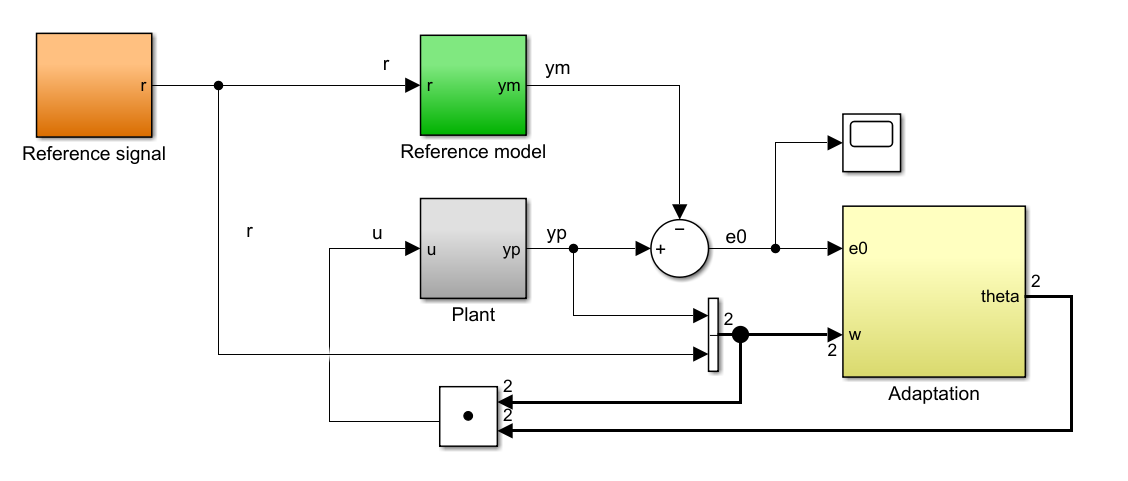
\includegraphics[width=0.8\textwidth]{img/diagrama_mrac_direto.png}
  \caption{Diagrama de blocos geral do controle MRAC direto.}
  \label{fig:mrac_direto}
\end{figure}

A Figura~\ref{fig:mrac_direto} mostra a arquitetura geral do controlador MRAC direto. O objetivo do sistema é ajustar os parâmetros do controlador de modo que a saída da planta acompanhe a saída do modelo de referência para qualquer entrada $r(t)$. O sinal de erro $e = y - y_m$ é utilizado para atualizar os parâmetros adaptativos.

\begin{figure}[h!]
  \centering
  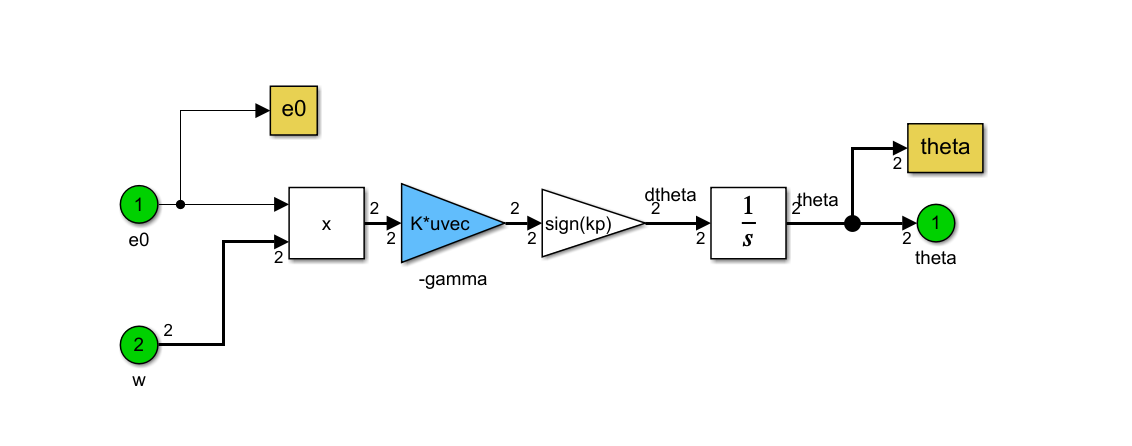
\includegraphics[width=0.6\textwidth]{img/diagrama_adaptacao.png}
  \caption{Malha de adaptação dos parâmetros $\bm{\theta}$.}
  \label{fig:adaptacao}
\end{figure}

Na Figura~\ref{fig:adaptacao}, destacamos a malha de adaptação, responsável por ajustar os parâmetros do controlador $\bm{\theta}$ com base no erro de seguimento. Essa adaptação ocorre conforme uma lei de atualização derivada da função de Lyapunov, garantindo estabilidade do sistema.

\begin{figure}[h!]
  \centering
  \begin{subfigure}[b]{0.32\textwidth}
    \centering
    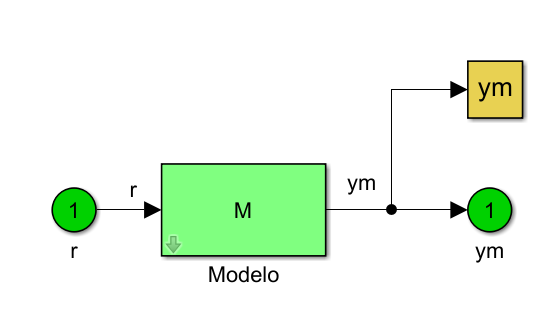
\includegraphics[width=\textwidth]{img/diagrama_modelo.png}
    \caption{Modelo de referência}
    \label{fig:modelo_referencia}
  \end{subfigure}
  \hfill
  \begin{subfigure}[b]{0.32\textwidth}
    \centering
    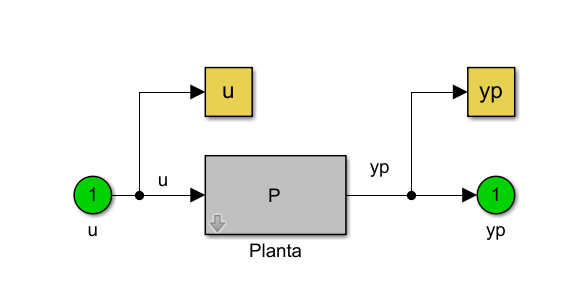
\includegraphics[width=\textwidth]{img/diagrama_planta.png}
    \caption{Planta controlada}
    \label{fig:planta}
  \end{subfigure}
  \hfill
  \begin{subfigure}[b]{0.32\textwidth}
    \centering
    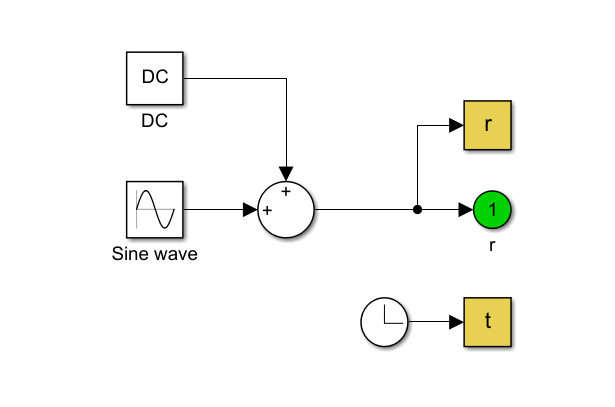
\includegraphics[width=\textwidth]{img/diagrama_referencia.png}
    \caption{Sinal de referência $r(t)$}
    \label{fig:referencia}
  \end{subfigure}
  \caption{Componentes individuais do sistema MRAC.}
  \label{fig:componentes_mrac}
\end{figure}

A Figura~\ref{fig:componentes_mrac} agrupa os blocos fundamentais do sistema MRAC. À esquerda, o modelo de referência define a dinâmica desejada para o sistema. Ao centro, está a planta controlada, que deve seguir essa referência. À direita, o sinal de referência $r(t)$ atua como entrada comum para ambos os blocos, sendo a base para comparação entre o comportamento ideal e o real.

\section{Resultados das simulações}

Cada subseção a seguir apresenta a configuração do experimento, espaço reservado para os dados obtidos em cada simulação e comentários sobre o desempenho do MRAC Direto.

\newpage

\subsection{Simulação \#1}
\subsubsection{Configuração do experimento:}
\begin{itemize}
\item \textbf{Planta:} $P(s) = \dfrac{k_p}{s - a_p} = \dfrac{1}{s - 2}$
\item \textbf{Modelo de referência:} $M(s) = \dfrac{k_m}{s + a_m} = \dfrac{1}{s + 1}$
\item \textbf{Condições iniciais:} $y_p(0)=0$, $y_m(0)=0$
\item \textbf{Sinal de referência:} DC = 1 (constante), $A_s=0$, $\omega_s=5$ rad/s
\item \textbf{Ganho de matching ótimo:} $\theta^* = \bigl[-(a_p + a_m)/k_p;k_m/k_p\bigr] = [-3;1]$
\item \textbf{Ganho de adaptação:} $\Gamma_1 = 2I_{2\times2}$, $\Gamma_2 = 100 I_{2\times2}$
\item \textbf{Condição inicial do parâmetro:} $\theta(0) = [0;0]$
\end{itemize}

\subsubsection{Resultados da simulação:}

\begin{figure}[h!]
    \centering
    \begin{subfigure}[b]{0.3\textwidth}
        \centering
        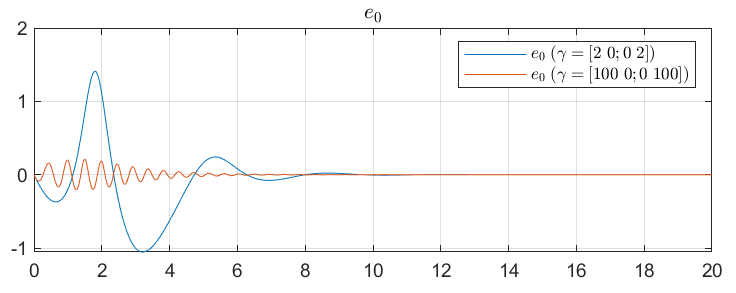
\includegraphics[width=\textwidth]{img/fig01a.png}
        \caption{Erro de Rastreamento}
    \end{subfigure}
    \begin{subfigure}[b]{0.3\textwidth}
        \centering
        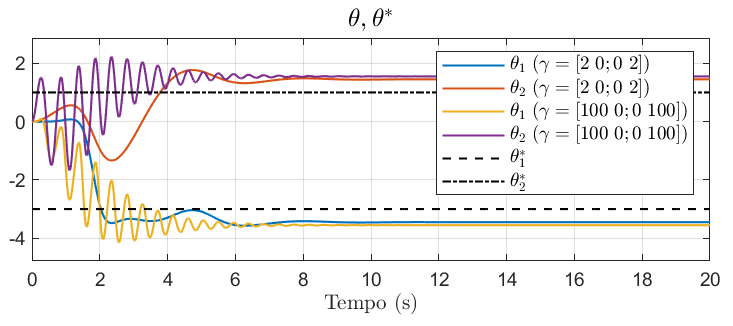
\includegraphics[width=\textwidth]{img/fig01b.png}
        \caption{Ganho de Adaptação}
    \end{subfigure}

    \begin{subfigure}[b]{0.3\textwidth}
        \centering
        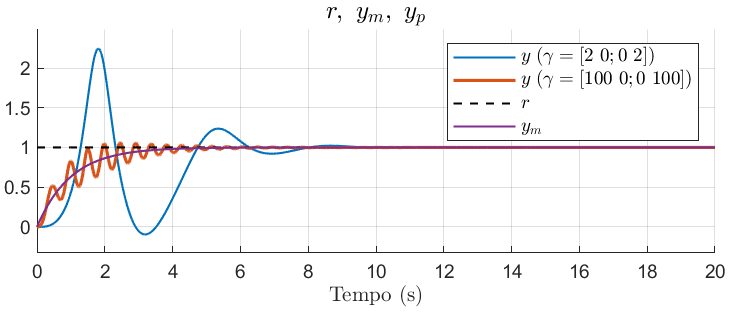
\includegraphics[width=\textwidth]{img/fig01c.png}
        \caption{Resposta do Sistema}
    \end{subfigure}
    \begin{subfigure}[b]{0.3\textwidth}
        \centering
        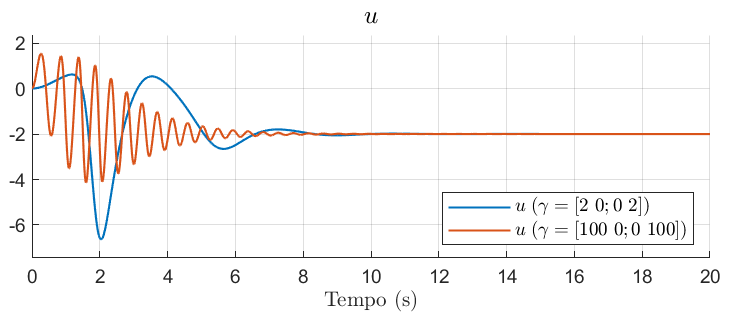
\includegraphics[width=\textwidth]{img/fig01e.png}
        \caption{Sinal de Controle}
    \end{subfigure}

    \begin{subfigure}[b]{0.3\textwidth}
        \centering
        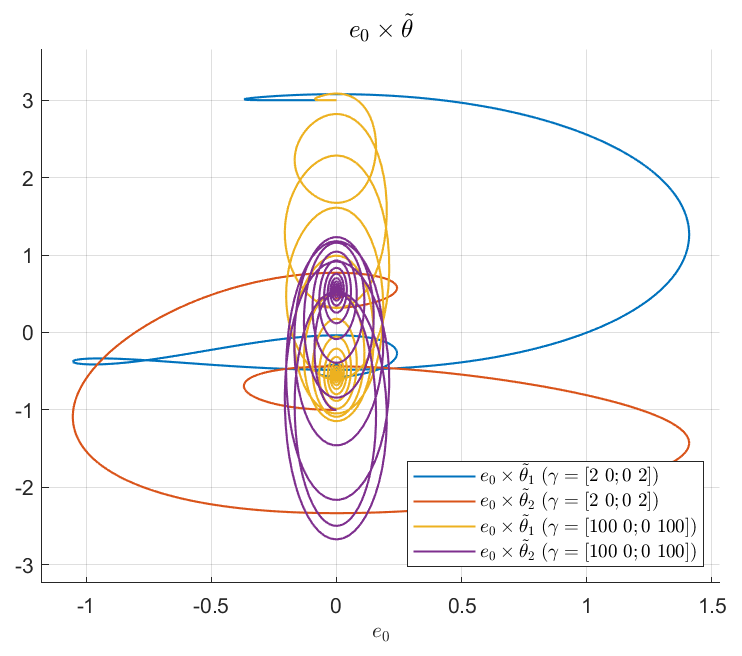
\includegraphics[width=\textwidth]{img/fig01d.png}
        \caption{Diagrama $e_0 \times \tilde{\theta}$}
    \end{subfigure}

    \caption{Resultado da simulação (Script: \textit{simu01.m})}
    \label{fig:sim1}
\end{figure}

\subsubsection{Comentários:}

A simulação do MRAC Direto apresentou os seguintes comportamentos, conforme a variação do ganho de adaptação $\Gamma$:

\begin{itemize}
    \item \textbf{Erro de rastreamento ($e_0$):} Para $\Gamma = 100I$, o erro converge mais rapidamente com menor overshoot. Já para $\Gamma = 2I$, a convergência é mais lenta e com maiores oscilações, só que uma menor frequência de oscilação.

    \item \textbf{Ganho de adaptação ($\theta$):} Ambos os casos não convergem para o valor ótimo $\theta^* = [-3;1]$. Porque o sinal de entrada que é um sinal DC igual a 1, o que não auxilia na convergência do ganho de adaptação.

    \item \textbf{Resposta do sistema ($y_p$ e $y_m$):} O rastreamento da referência é mais eficiente para $\Gamma = 100I$, apresentando menor erro e resposta mais rápida.

    \item \textbf{Sinal de controle ($u$):} Ambos os casos convergem para o valor adequado em regime permanente. Com $\Gamma = 100I$, o controle atua de forma mais intensa no início, mas estabiliza mais rapidamente.

    \item \textbf{Diagrama de fase ($e_0 \times \tilde{\theta}$):} Para $\Gamma = 2I$, a trajetória é mais lenta e ampla; para $\Gamma = 100I$, há convergência rápida com órbitas mais fechadas.

\end{itemize}

\textbf{Conclusão:} Aumentar o ganho de adaptação $\Gamma$ melhora significativamente a velocidade de convergência do sistema, tanto para o erro quanto para os parâmetros adaptativos, ao custo de maior agressividade no transiente.

\newpage

\subsection{Simulação \#2}
\subsubsection{Configuração do experimento:}
\begin{itemize}
\item \textbf{Planta:} $P(s) = \dfrac{1}{s - 2}$
\item \textbf{Modelo de referência:} $M(s) = \dfrac{1}{s + 1}$
\item \textbf{Condições iniciais:} $y_p(0)=0$, $y_m(0)=0$
\item \textbf{Sinal de referência:} DC = 2 (constante), $A_s=1$, $\omega_s=5$ rad/s
\item \textbf{Ganho de matching ótimo:} $\theta^* = [-3;1]$
\item \textbf{Ganho de adaptação:} $\Gamma_1 = 2I_{2\times2}$, $\Gamma_2 = 100 I_{2\times2}$
\item \textbf{Condição inicial do parâmetro:} $\theta(0) = [0;0]$
\end{itemize}

\subsubsection{Resultados da simulação:}

\begin{figure}[h!]
    \centering
    \begin{subfigure}[b]{0.3\textwidth}
        \centering
        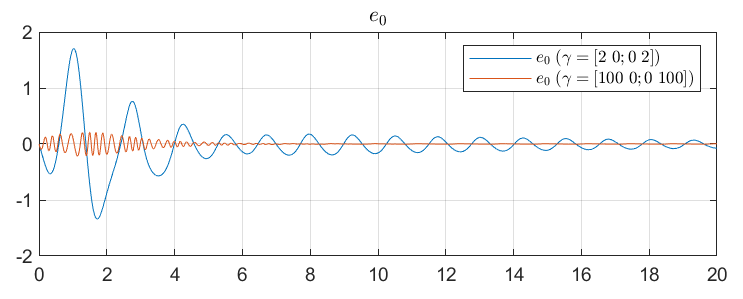
\includegraphics[width=\textwidth]{img/fig02a.png}
        \caption{Erro de Rastreamento}
    \end{subfigure}
    \begin{subfigure}[b]{0.3\textwidth}
        \centering
        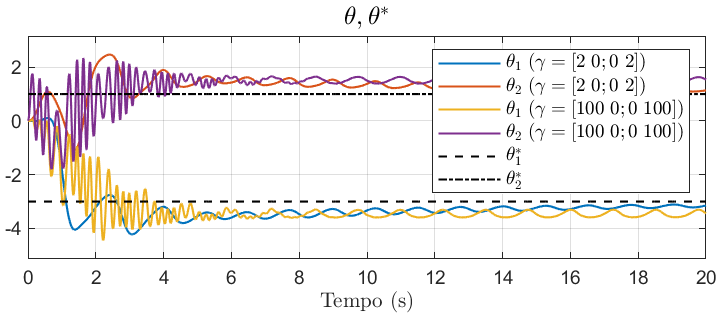
\includegraphics[width=\textwidth]{img/fig02b.png}
        \caption{Ganho de Adaptação}
    \end{subfigure}

    \begin{subfigure}[b]{0.3\textwidth}
        \centering
        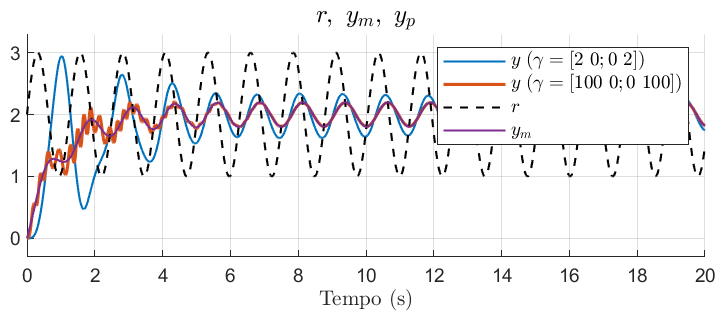
\includegraphics[width=\textwidth]{img/fig02c.png}
        \caption{Resposta do Sistema}
    \end{subfigure}
    \begin{subfigure}[b]{0.3\textwidth}
        \centering
        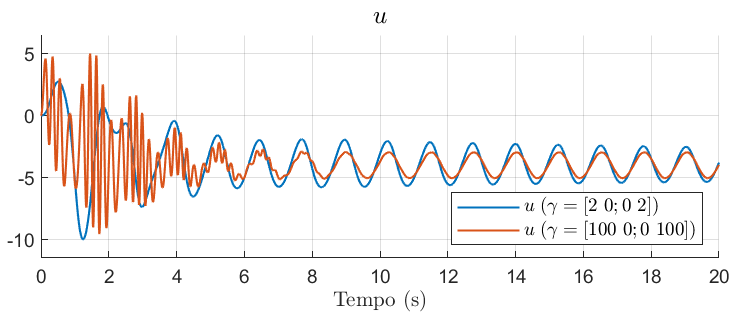
\includegraphics[width=\textwidth]{img/fig02e.png}
        \caption{Sinal de Controle}
    \end{subfigure}

    \begin{subfigure}[b]{0.3\textwidth}
        \centering
        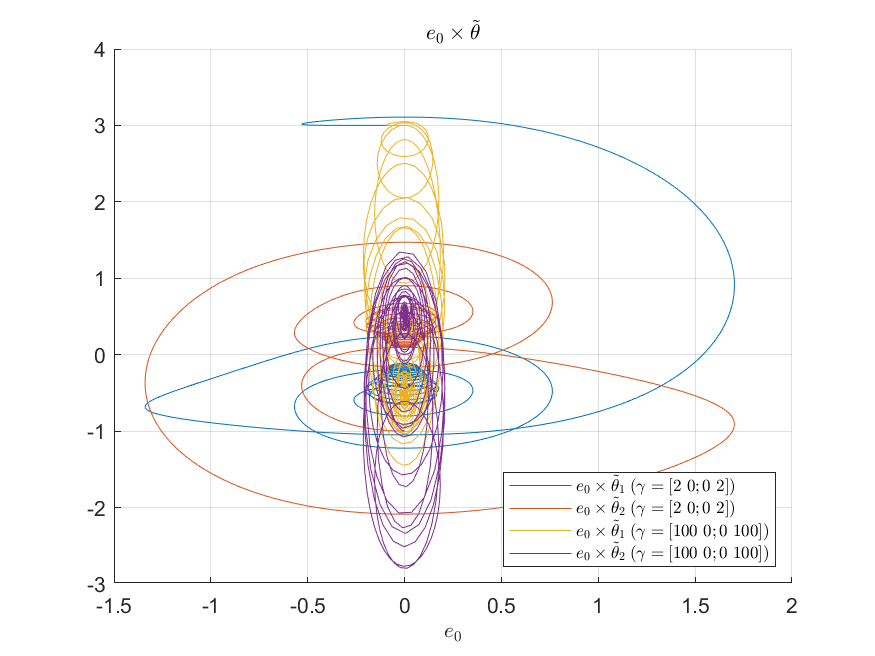
\includegraphics[width=\textwidth]{img/fig02d.png}
        \caption{Diagrama $e_0 \times \tilde{\theta}$}
    \end{subfigure}

    \caption{Resultado da simulação (Script: \textit{simu02.m})}
    \label{fig:sim2}
\end{figure}

\subsubsection{Comentários:}

Nesta simulação, foi utilizado um sinal de referência composto por uma componente DC e uma senoidal, o que introduz maior oscilação no sistema. Os principais resultados observados foram:

\begin{itemize}
    \item \textbf{Erro de rastreamento ($e_0$):} O erro apresenta comportamento oscilatório permanente devido à componente senoidal do sinal de referência. Com $\Gamma = 100I$, o erro é mais suavizado e acompanha melhor a referência.

    \item \textbf{Ganho de adaptação ($\theta$):} Ambos os casos convergem para valores próximos de $\theta^*$, com maior rapidez e menor variação para $\Gamma = 100I$.

    \item \textbf{Resposta do sistema ($y_p$, $y_m$, $r$):} A resposta com $\Gamma = 100I$ segue melhor a referência, com menor defasagem e melhor rastreamento da componente senoidal.

    \item \textbf{Sinal de controle ($u$):} Oscilatório em ambos os casos, com maior intensidade e frequência no início. A escolha de $\Gamma$ mais alto permite estabilização mais rápida, porém com maior ação de controle.

    \item \textbf{Diagrama de fase ($e_0 \times \tilde{\theta}$):} Com $\Gamma = 100I$, as trajetórias convergem de forma mais concentrada em torno da origem, indicando melhor desempenho adaptativo.

\end{itemize}

\textbf{Conclusão:} A presença da componente senoidal no sinal de referência exige maior capacidade adaptativa do sistema. O ganho de adaptação elevado ($\Gamma = 100I$) proporciona resposta mais precisa, embora com maior esforço de controle.

\newpage

\subsection{Simulação \#3}
\subsubsection{Configuração do experimento:}
\begin{itemize}
\item \textbf{Planta:} $P(s) = \dfrac{1}{s - 2}$
\item \textbf{Modelo de referência:} $M(s) = \dfrac{1}{s + 1}$
\item \textbf{Condições iniciais:} $y_p(0)=3$, $y_m(0)=0$
\item \textbf{Sinal de referência:} DC = 1 (constante), $A_s=0$, $\omega_s=5$,rad/s
\item \textbf{Ganho de matching ótimo:} $\theta^* = [-3;1]$
\item \textbf{Ganho de adaptação:} $\Gamma_1 = 2I_{2\times2}$, $\Gamma_2 = 100 I_{2\times2}$
\item \textbf{Condição inicial do parâmetro:} $\theta(0) = [0;0]$
\end{itemize}

\subsubsection{Resultados da simulação:}

\begin{figure}[h!]
    \centering
    \begin{subfigure}[b]{0.3\textwidth}
        \centering
        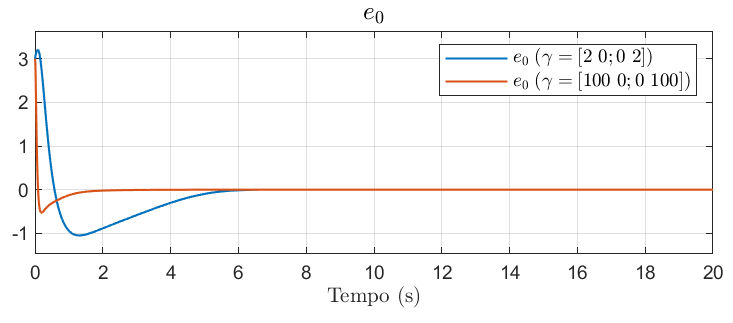
\includegraphics[width=\textwidth]{img/fig03a.png}
        \caption{Erro de Rastreamento}
    \end{subfigure}
    \begin{subfigure}[b]{0.3\textwidth}
        \centering
        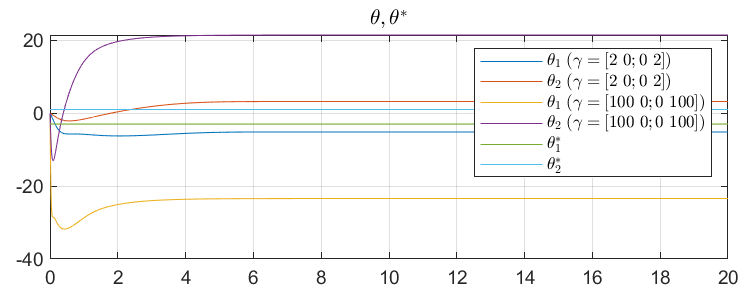
\includegraphics[width=\textwidth]{img/fig03b.png}
        \caption{Ganho de Adaptação}
    \end{subfigure}

    \begin{subfigure}[b]{0.3\textwidth}
        \centering
        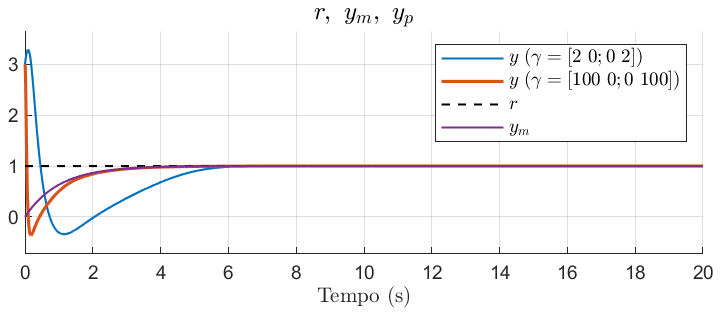
\includegraphics[width=\textwidth]{img/fig03c.png}
        \caption{Resposta do Sistema}
    \end{subfigure}
    \begin{subfigure}[b]{0.3\textwidth}
        \centering
        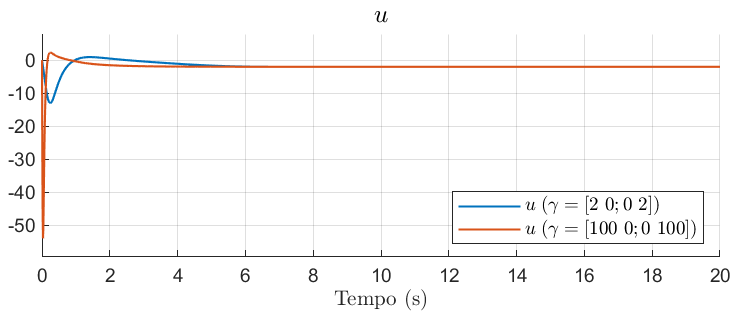
\includegraphics[width=\textwidth]{img/fig03e.png}
        \caption{Sinal de Controle}
    \end{subfigure}

    \begin{subfigure}[b]{0.3\textwidth}
        \centering
        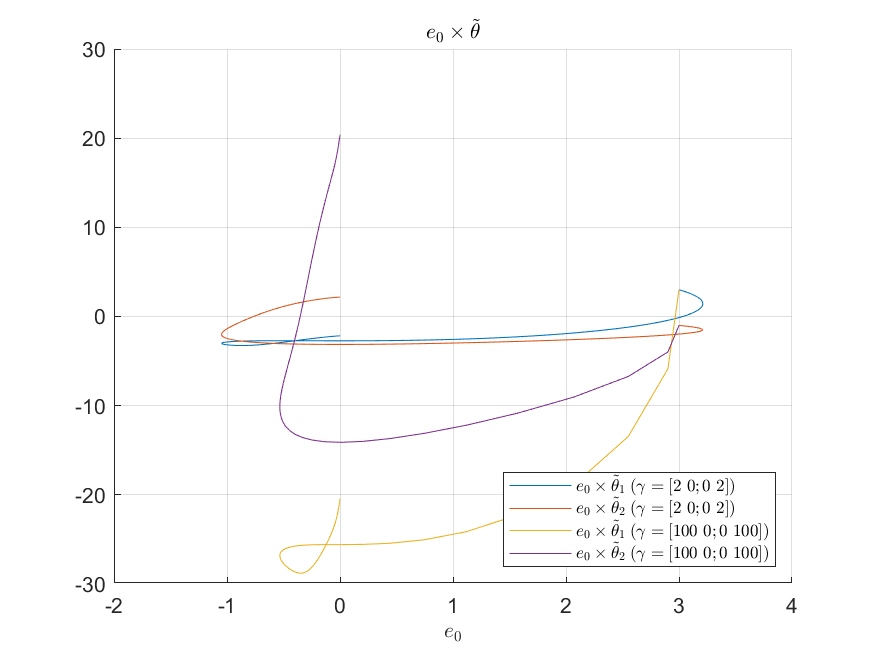
\includegraphics[width=\textwidth]{img/fig03d.png}
        \caption{Diagrama $e_0 \times \tilde{\theta}$}
    \end{subfigure}

    \caption{Resultado da simulação (Script: \textit{simu03.m})}
    \label{fig:sim3}
\end{figure}

\subsubsection{Comentários:}

Nesta simulação, a planta parte de uma condição inicial não nula ($y_p(0) = 3$), enquanto o modelo inicia em zero. O sinal de referência é constante (DC = 1). Os principais resultados observados foram:

\begin{itemize}
    \item \textbf{Erro de rastreamento ($e_0$):} O erro converge rapidamente para zero, sendo mais eficiente para $\Gamma = 100I$. A presença do offset inicial é corrigida com maior rapidez neste caso.

    \item \textbf{Ganho de adaptação ($\theta$):} Os parâmetros adaptativos se ajustam rapidamente e não estabilizam em torno de $\theta^*$, com menor oscilação e adaptação mais rápida para maior ganho de adaptação.

    \item \textbf{Resposta do sistema:} O sistema com $\Gamma = 100I$ segue o modelo de referência com mais precisão, apresentando menor tempo de acomodação e sobre-elevação.

    \item \textbf{Sinal de controle ($u$):} O controle é inicialmente intenso devido à diferença nas condições iniciais. Para $\Gamma = 100I$, observa-se maior esforço de controle, mas com resposta mais eficaz.

    \item \textbf{Diagrama de fase ($e_0 \times \tilde{\theta}$):} As trajetórias convergem rapidamente para a origem, especialmente para $\Gamma = 100I$, indicando uma adaptação eficiente mesmo com condições iniciais desfavoráveis.

\end{itemize}

\textbf{Conclusão:} A diferença nas condições iniciais evidencia a importância do ganho de adaptação. Valores maiores de $\Gamma$ resultam em respostas mais rápidas e precisas, compensando rapidamente desvios iniciais.

\newpage

\subsection{Simulação \#4}
\subsubsection{Configuração do experimento:}
\begin{itemize}
\item \textbf{Planta:} $P(s) = \dfrac{1}{s - 2}$
\item \textbf{Modelo de referência:} $M(s) = \dfrac{1}{s + 1}$
\item \textbf{Condições iniciais:} $y_p(0)=3$, $y_m(0)=0$
\item \textbf{Sinal de referência:} DC = 2 (constante), $A_s=1$, $\omega_s=5$,rad/s
\item \textbf{Ganho de matching ótimo:} $\theta^* = [-3;1]$
\item \textbf{Ganho de adaptação:} $\Gamma_1 = 2I_{2\times2}$, $\Gamma_2 = 100 I_{2\times2}$
\item \textbf{Condição inicial do parâmetro:} $\theta(0) = [0;0]$
\end{itemize}

\subsubsection{Resultados da simulação:}

\begin{figure}[h!]
    \centering
    \begin{subfigure}[b]{0.3\textwidth}
        \centering
        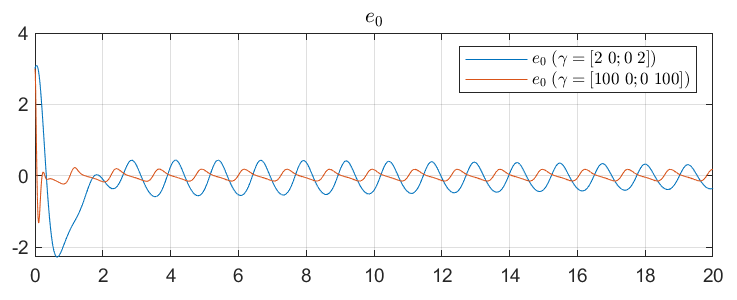
\includegraphics[width=\textwidth]{img/fig04a.png}
        \caption{Erro de Rastreamento}
    \end{subfigure}
    \begin{subfigure}[b]{0.3\textwidth}
        \centering
        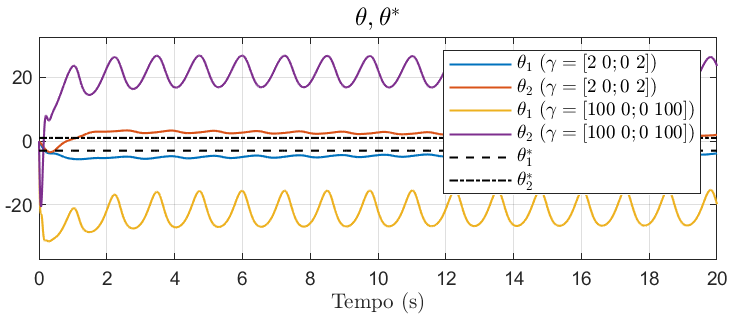
\includegraphics[width=\textwidth]{img/fig04b.png}
        \caption{Ganho de Adaptação}
    \end{subfigure}

    \begin{subfigure}[b]{0.3\textwidth}
        \centering
        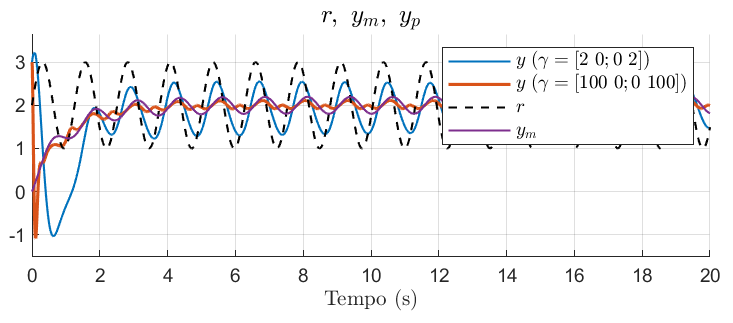
\includegraphics[width=\textwidth]{img/fig04c.png}
        \caption{Resposta do Sistema}
    \end{subfigure}
    \begin{subfigure}[b]{0.3\textwidth}
        \centering
        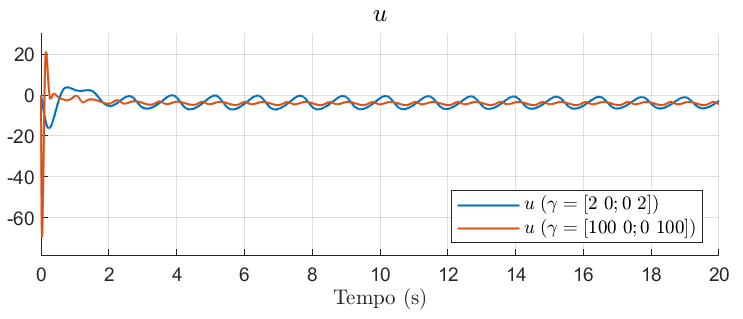
\includegraphics[width=\textwidth]{img/fig04e.png}
        \caption{Sinal de Controle}
    \end{subfigure}

    \begin{subfigure}[b]{0.3\textwidth}
        \centering
        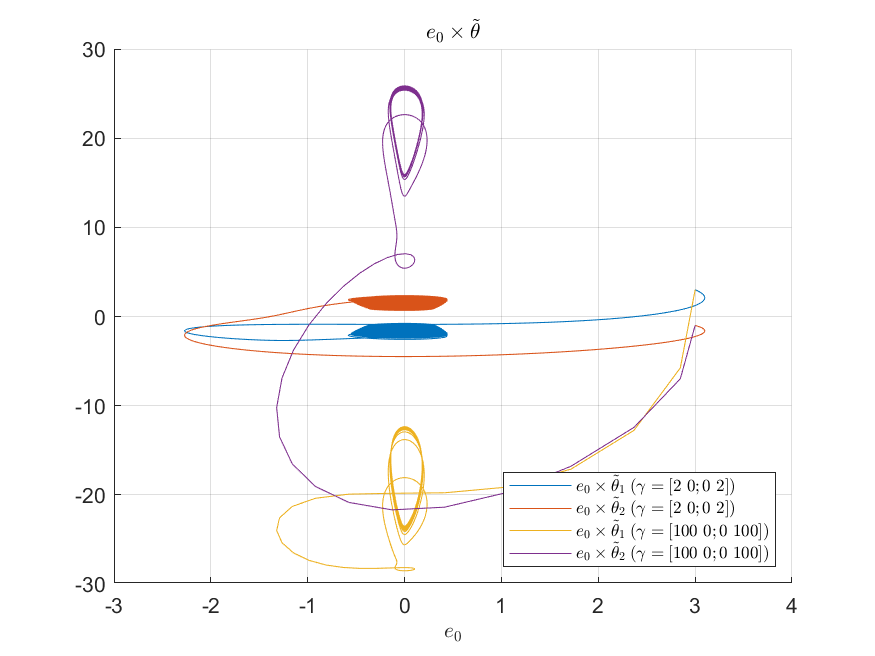
\includegraphics[width=\textwidth]{img/fig04d.png}
        \caption{Diagrama $e_0 \times \tilde{\theta}$}
    \end{subfigure}

    \caption{Resultado da simulação (Script: \textit{simu04.m})}
    \label{fig:sim4}
\end{figure}

\subsubsection{Comentários:}

Nesta simulação, a planta inicia novamente em $y_p(0)=3$, mas o sinal de referência inclui uma componente senoidal além da parte DC ($DC=2$, $A_s=1$, $\omega_s=5$ rad/s). Isso introduz um regime permanente oscilatório. Os principais pontos observados são:

\begin{itemize}
    \item \textbf{Erro de rastreamento ($e_0$):} O erro não converge para zero devido à presença do componente harmônico no sinal de referência. No entanto, para $\Gamma = 100I$, o erro apresenta menor amplitude de oscilação, indicando melhor desempenho de rastreamento.

    \item \textbf{Ganho de adaptação ($\theta$):} Os parâmetros adaptativos não convergem para valores constantes, pois o sistema está em regime oscilatório. Ainda assim, os ganhos oscilam em torno de valores próximos de $\theta^*$ no caso de $\Gamma = 2I$, com maior oscilação observada para $\Gamma = 100I$.

    \item \textbf{Resposta do sistema:} O sistema com maior ganho de adaptação responde mais rapidamente e com menor erro de seguimento da referência. Entretanto, a presença de altas frequências exige maior esforço adaptativo.

    \item \textbf{Sinal de controle ($u$):} O controle apresenta oscilações significativas para ambas as configurações, mas mais intensas para $\Gamma = 100I$, refletindo a tentativa de acompanhar a componente senoidal do sinal de referência.

    \item \textbf{Diagrama de fase ($e_0 \times \tilde{\theta}$):} As trajetórias não convergem para a origem, como esperado em um regime não estacionário. Os ciclos fechados no plano de fase revelam a persistência da oscilação e o comportamento quase-periódico da adaptação.

\end{itemize}

\textbf{Conclusão:} A introdução da componente senoidal no sinal de referência impossibilita a convergência do erro para zero. Ainda assim, o aumento do ganho de adaptação melhora o desempenho de rastreamento, ao custo de maior esforço de controle e maiores oscilações nos parâmetros adaptativos.

\newpage

\subsection{Simulação \#5}
\subsubsection{Configuração do experimento:}
\begin{itemize}
\item \textbf{Planta:} $P(s) = \dfrac{1}{s - 2}$
\item \textbf{Modelo de referência:} $M(s) = \dfrac{1}{s + 10}$
\item \textbf{Condições iniciais:} $y_p(0)=0$, $y_m(0)=0$
\item \textbf{Sinal de referência:} DC = 1 (constante), $A_s=0$, $\omega_s=5$,rad/s
\item \textbf{Ganho de matching ótimo:} $\theta^* = [-(2+10)/1;1/1] = [-12;1]$
\item \textbf{Ganho de adaptação:} $\Gamma_1 = 2I_{2\times2}$, $\Gamma_2 = 100 I_{2\times2}$
\item \textbf{Condição inicial do parâmetro:} $\theta(0) = [0;0]$
\end{itemize}

\subsubsection{Resultados da simulação:}

\begin{figure}[h!]
    \centering
    \begin{subfigure}[b]{0.3\textwidth}
        \centering
        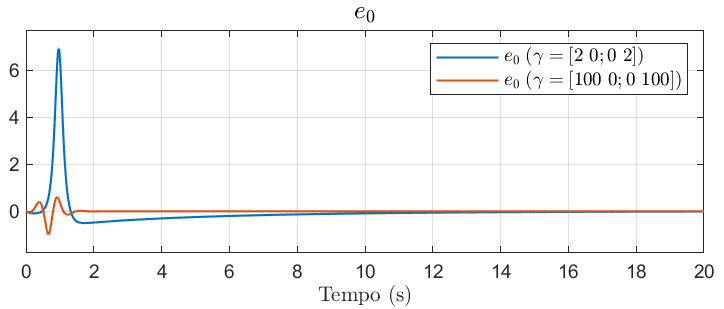
\includegraphics[width=\textwidth]{img/fig05a.png}
        \caption{Erro de Rastreamento}
    \end{subfigure}
    \begin{subfigure}[b]{0.3\textwidth}
        \centering
        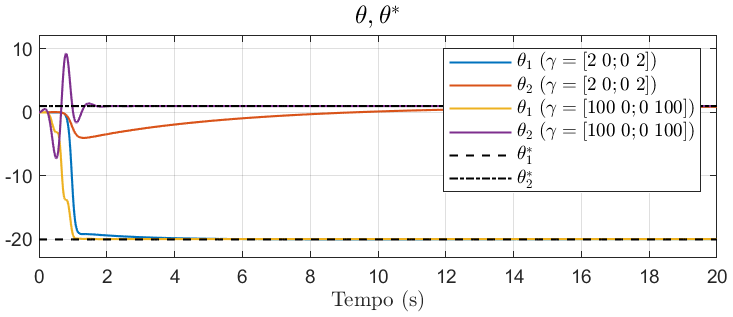
\includegraphics[width=\textwidth]{img/fig05b.png}
        \caption{Ganho de Adaptação}
    \end{subfigure}

    \begin{subfigure}[b]{0.3\textwidth}
        \centering
        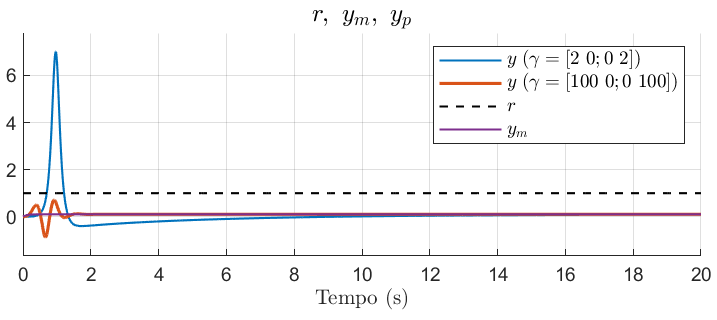
\includegraphics[width=\textwidth]{img/fig05c.png}
        \caption{Resposta do Sistema}
    \end{subfigure}
    \begin{subfigure}[b]{0.3\textwidth}
        \centering
        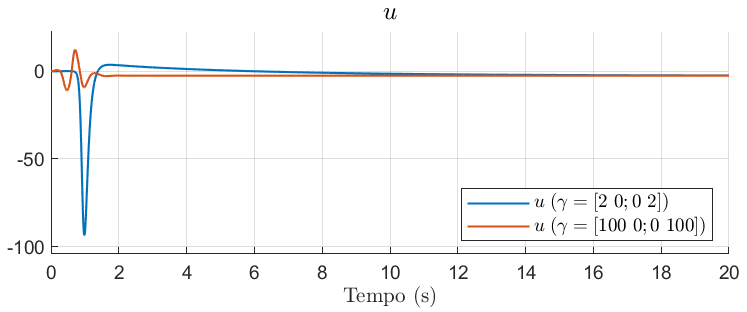
\includegraphics[width=\textwidth]{img/fig05e.png}
        \caption{Sinal de Controle}
    \end{subfigure}

    \begin{subfigure}[b]{0.3\textwidth}
        \centering
        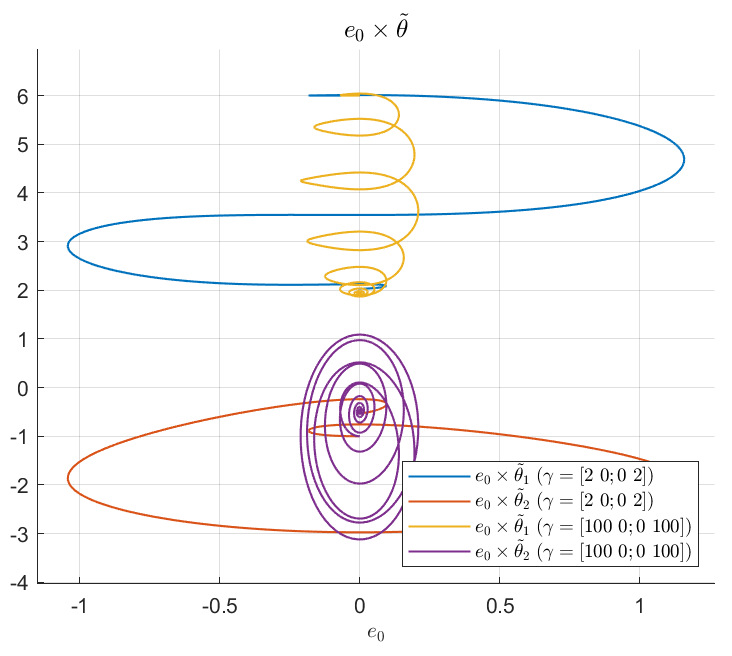
\includegraphics[width=\textwidth]{img/fig05d.png}
        \caption{Diagrama $e_0 \times \tilde{\theta}$}
    \end{subfigure}

    \caption{Resultado da simulação (Script: \textit{simu05.m})}
    \label{fig:sim5}
\end{figure}

\subsubsection{Comentários:}

Nesta simulação, o modelo de referência foi modificado para $M(s) = \frac{1}{s+10}$, ou seja, com constante de tempo menor devido ao aumento de $a_m$ de 1 para 10. O sinal de referência é puramente constante ($DC = 1$), sem componente senoidal, o que permite avaliar o comportamento do sistema em regime estacionário. Os principais pontos observados são:

\begin{itemize}
    \item \textbf{Erro de rastreamento ($e_0$):} Em Figura~\ref{fig:sim5}(a),  erro converge para zero em ambos os casos. Para $\Gamma = 2I$, observa-se um pico inicial mais acentuado. Já com $\Gamma = 100I$, a convergência é mais rápida e uma pequena ondulação em torno de $t \approx 1\,$s, com menor overshoot.

    \item \textbf{Ganho de adaptação ($\theta$):} Em Figura~\ref{fig:sim5}(b), os parâmetros adaptativos convergem para valores constantes em ambos os casos, aproximando-se de $\theta^* = [-12,\;1]$. A configuração com $\Gamma = 100I$ apresenta convergência mais rápida, com oscilações transitórias ligeiramente maiores. Para $\Gamma = 2I$, a convergência é mais lenta e apresenta maior oscilação inicial.

    \item \textbf{Resposta do sistema:} Em Figura~\ref{fig:sim5}(c), a resposta com $\Gamma = 100I$ é mais rápida e atinge o valor de regime de forma mais direta. Já para $\Gamma = 2I$, o sistema apresenta overshoot antes de se estabilizar.

    \item \textbf{Sinal de controle ($u$):} Em Figura~\ref{fig:sim5}(d), o controle apresenta um pico mais elevado no caso de $\Gamma = 2I$, chegando a aproximadamente $-90$, enquanto para $\Gamma = 100I$ o pico é menor (em torno de $-10$ e $10$). Após o regime transitório, ambos convergem para valores próximos.

    \item \textbf{Diagrama de fase ($e_0 \times \tilde{\theta}$):} Em Figura~\ref{fig:sim5}(e),As trajetórias no plano de fase convergem para a origem em ambos os casos, indicando estabilidade e boa adaptação. Para $\Gamma = 2I$, os ciclos iniciais são mais amplos e com espirais mais prolongadas. Já com $\Gamma = 100I$, a convergência é mais direta e rápida.

\end{itemize}

\textbf{Conclusão:} O aumento do ganho de adaptação ($\Gamma = 100I$) acelera a convergência do erro e dos parâmetros adaptativos, com menor overshoot e menor esforço de controle durante o transitório, entretanto com um comportamento mais oscilatório. Ganhos menores ($\Gamma = 2I$) resultam em comportamento mais lento e maior pico de controle, apesar de também garantir rastreamento preciso. Em ambos os casos, o controlador estabiliza a planta instável $P(s)=\frac{1}{s-2}$ e segue adequadamente o modelo de referência $M(s)=\frac{1}{s+10}$.

\newpage

\subsection{Simulação \#6}
\subsubsection{Configuração do experimento:}
\begin{itemize}
\item \textbf{Planta:} $P(s) = \dfrac{1}{s - 2}$
\item \textbf{Modelo de referência:} $M(s) = \dfrac{1}{s + 10}$
\item \textbf{Condições iniciais:} $y_p(0)=0$, $y_m(0)=0$
\item \textbf{Sinal de referência:} DC = 2, $A_s=1$, $\omega_s=5$ rad/s
\item \textbf{Ganho de matching ótimo:} $\theta^* = [-(2+10)/1;2/1] = [-12;2]$
\item \textbf{Ganho de adaptação:} $\Gamma_1 = 2I_{2\times2}$, $\Gamma_2 = 100I_{2\times2}$
\item \textbf{Condição inicial do parâmetro:} $\theta(0) = [0;0]$
\end{itemize}

\subsubsection{Resultados da simulação:}

\begin{figure}[h!]
    \centering
    \begin{subfigure}[b]{0.3\textwidth}
        \centering
        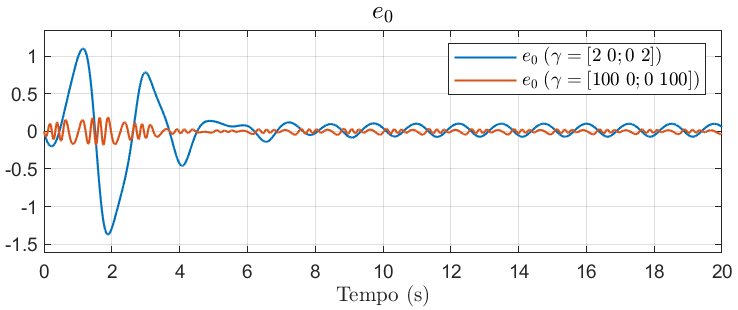
\includegraphics[width=\textwidth]{img/fig06a.png}
        \caption{Erro de Rastreamento}
    \end{subfigure}
    \begin{subfigure}[b]{0.3\textwidth}
        \centering
        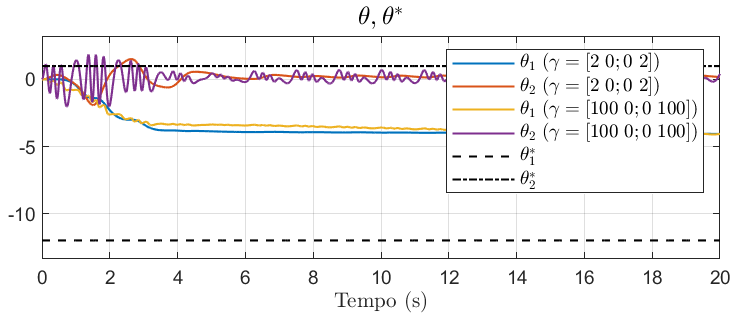
\includegraphics[width=\textwidth]{img/fig06b.png}
        \caption{Ganho de Adaptação}
    \end{subfigure}

    \begin{subfigure}[b]{0.3\textwidth}
        \centering
        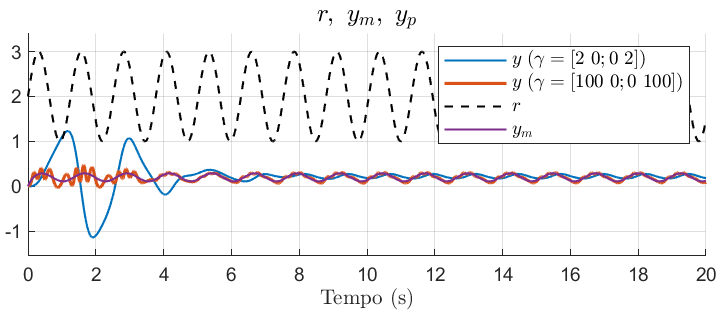
\includegraphics[width=\textwidth]{img/fig06c.png}
        \caption{Resposta do Sistema}
    \end{subfigure}
    \begin{subfigure}[b]{0.3\textwidth}
        \centering
        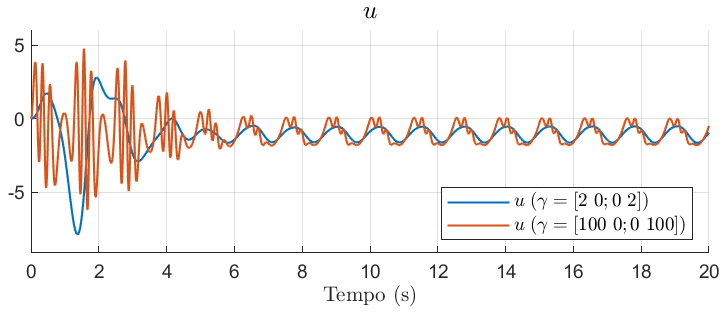
\includegraphics[width=\textwidth]{img/fig06e.png}
        \caption{Sinal de Controle}
    \end{subfigure}

    \begin{subfigure}[b]{0.3\textwidth}
        \centering
        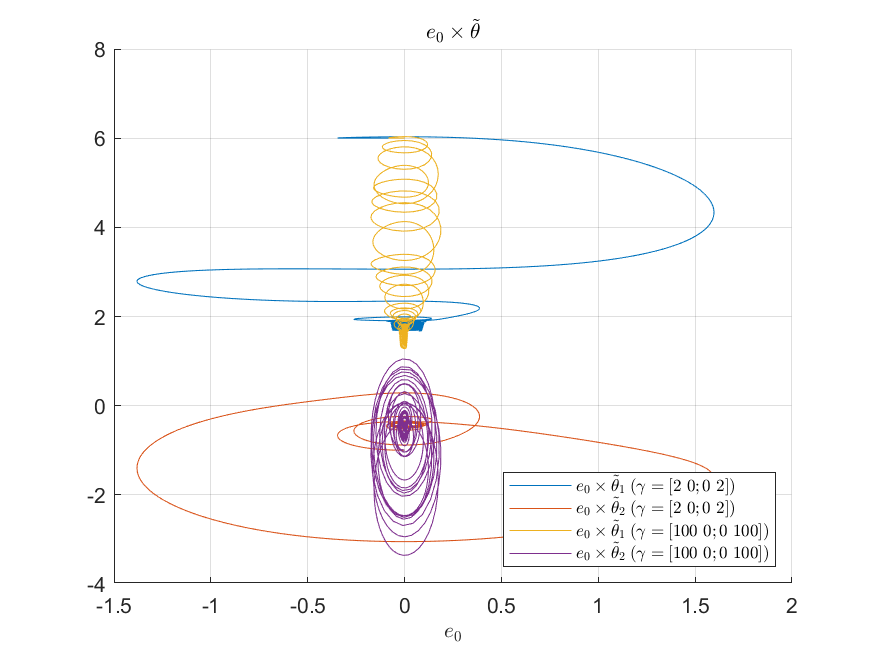
\includegraphics[width=\textwidth]{img/fig06d.png}
        \caption{Diagrama $e_0 \times \tilde{\theta}$}
    \end{subfigure}

    \caption{Resultado da simulação (Script: \textit{simu06.m})}
    \label{fig:sim6}
\end{figure}

\subsubsection{Comentários:}

Nesta simulação, o modelo de referência é $M(s) = \frac{1}{s+10}$ (com $a_m=10$), e o sinal de referência possui componente senoidal sobreposta à parte DC ($DC = 2$, $A_s = 1$, $\omega_s = 5\,$rad/s). Dessa forma, o sistema entra em regime permanente oscilatório. Os principais pontos observados são:

\begin{itemize}
    \item \textbf{Erro de rastreamento ($e_0$):} Em Figura~\ref{fig:sim6}(a), o erro não converge para zero devido à presença da componente harmônica no referencial. Para $\Gamma = 2I$ (azul), as oscilações iniciais de $e_0$ são maiores e demoram mais a se estabilizar; já para $\Gamma = 100I$ (laranja), o erro atinge menor amplitude e adquire regime permanente oscilatório mais rapidamente, indicando melhor desempenho de seguimento.

    \item \textbf{Ganho de adaptação ($\theta$):} Em Figura~\ref{fig:sim6}(b), ambos os parâmetros $\theta_1$ e $\theta_2$ não convergem a constantes fixas, pois permanecem oscilando para acompanhar o referencial senoidal. Para $\Gamma = 100I$, as oscilações transitórias em $\theta$ são mais intensas e a adaptação entra em regime oscilatório mais cedo, enquanto para $\Gamma = 2I$ a variação é mais lenta, mas também menos amortecida.

    \item \textbf{Resposta do sistema ($y$, $y_m$, $r$):} Em Figura~\ref{fig:sim6}(c), a saída de referência $r(t) = 2 + \sin(5\,t)$ (linha preta tracejada) é seguida pela saída do modelo $y_m$ (rosa). Para $\Gamma = 100I$, $y(t)$ (laranja) aproxima-se de $y_m$ com menor defasagem e amplitude de erro reduzida, entrando rapidamente em regime permanente. Para $\Gamma = 2I$, $y(t)$ (azul) segue $y_m$ com overshoot maior e mais defasagem, levando mais tempo até estabilizar no padrão oscilatório.

    \item \textbf{Sinal de controle ($u$):} Em Figura~\ref{fig:sim6}(d), observa-se que $\Gamma = 100I$ (laranja) gera um pico de controle inicial maior (na ordem de $\pm 5$), mas as oscilações em regime permanente têm amplitude menor. Para $\Gamma = 2I$ (azul), o pico inicial é mais baixo, porém as oscilações de $u(t)$ em regime permanente permanecem de maior amplitude, refletindo a dificuldade de acompanhar plenamente a parte harmônica.

    \item \textbf{Diagrama de fase ($e_0 \times \tilde{\theta}$):} Em Figura~\ref{fig:sim6}(e), as trajetórias não convergem para a origem, pois o erro e o vetor de erro de parâmetros $\tilde{\theta} = \theta - \theta^*$ permanecem oscilando em torno de valores médios. Para $\Gamma = 2I$ (azul), as espirais no plano de fase são mais amplas e demoram mais para adotar um padrão quase-periódico; já para $\Gamma = 100I$ (laranja), a trajetória atinge rapidamente um ciclo quase-periódico de menor amplitude, indicando regime oscilatório mais estável.
\end{itemize}

\textbf{Conclusão:} A inclusão da componente senoidal no sinal de referência impede a convergência do erro para zero. O ganho de adaptação mais alto ($\Gamma = 100I$) resulta em melhor desempenho de rastreamento em regime permanente (menor amplitude de erro e de oscilações nos parâmetros), porém exige maior esforço inicial de controle e gera oscilações mais rápidas em $\theta$. O ganho menor ($\Gamma = 2I$) leva a oscilações iniciais mais amplas e maior defasagem, ainda que com menor agressividade no sinal de controle. Em ambos os casos, o controlador adaptativo estabiliza a planta instável $P(s)=\frac{1}{s-2}$ e acompanha adequadamente o modelo de referência $M(s)=\frac{1}{s+10}$ em regime oscilatório.

\newpage

\subsection{Simulação \#7}
\subsubsection{Configuração do experimento:}
\begin{itemize}
\item \textbf{Planta:} $P(s) = \dfrac{1}{s - 2}$
\item \textbf{Modelo de referência:} $M(s) = \dfrac{10}{s + 1}$
\item \textbf{Condições iniciais:} $y_p(0)=0$, $y_m(0)=0$
\item \textbf{Sinal de referência:} DC = 1, $A_s=0$, $\omega_s=5$ rad/s
\item \textbf{Ganho de matching ótimo:} $\theta^* = [-(2+1)/1;10/1] = [-3;10]$
\item \textbf{Ganho de adaptação:} $\Gamma_1 = 2I_{2\times2}$, $\Gamma_2 = 100I_{2\times2}$
\item \textbf{Condição inicial do parâmetro:} $\theta(0) = [0;0]$
\end{itemize}

\subsubsection{Resultados da simulação:}

\begin{figure}[h!]
    \centering
    \begin{subfigure}[b]{0.3\textwidth}
        \centering
        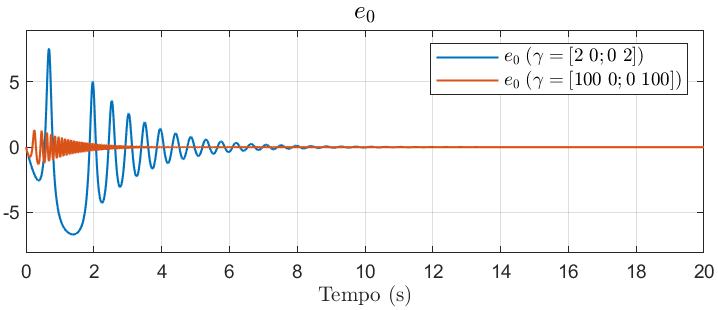
\includegraphics[width=\textwidth]{img/fig07a.png}
        \caption{Erro de Rastreamento}
    \end{subfigure}
    \begin{subfigure}[b]{0.3\textwidth}
        \centering
        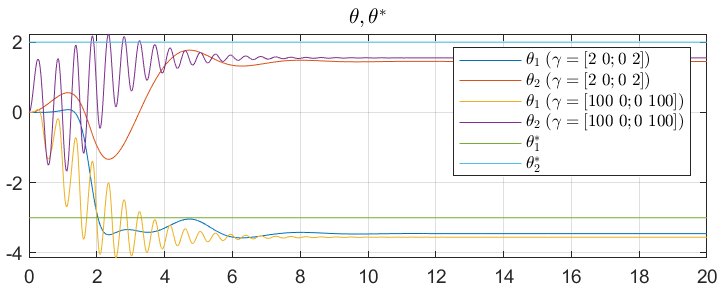
\includegraphics[width=\textwidth]{img/fig07b.png}
        \caption{Ganho de Adaptação}
    \end{subfigure}

    \begin{subfigure}[b]{0.3\textwidth}
        \centering
        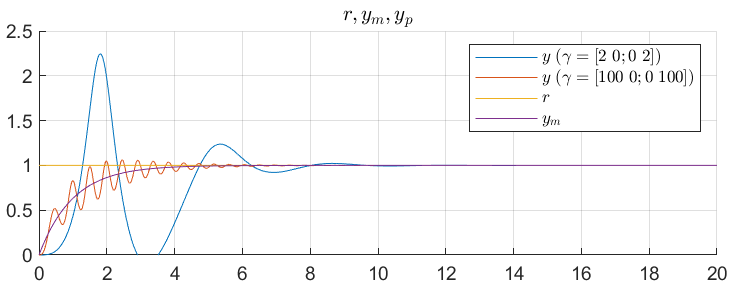
\includegraphics[width=\textwidth]{img/fig07c.png}
        \caption{Resposta do Sistema}
    \end{subfigure}
    \begin{subfigure}[b]{0.3\textwidth}
        \centering
        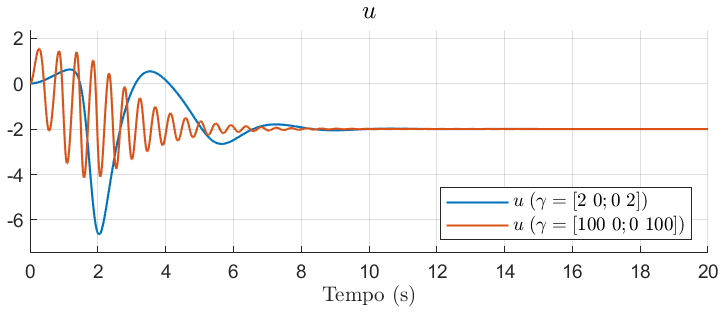
\includegraphics[width=\textwidth]{img/fig07e.png}
        \caption{Sinal de Controle}
    \end{subfigure}

    \begin{subfigure}[b]{0.3\textwidth}
        \centering
        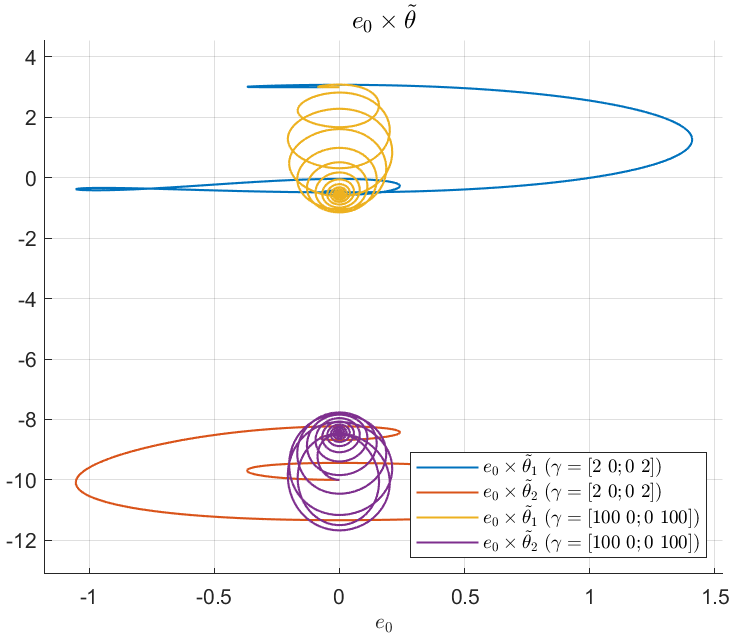
\includegraphics[width=\textwidth]{img/fig07d.png}
        \caption{Diagrama $e_0 \times \tilde{\theta}$}
    \end{subfigure}

    \caption{Resultado da simulação (Script: \textit{simu07.m})}
    \label{fig:sim7}
\end{figure}

\subsubsection{Comentários:}

Nesta simulação, o modelo de referência é dado por $M(s) = \frac{10}{s+1}$, ou seja, uma planta de primeira ordem com ganho estático maior (10) e constante de tempo igual a 1, mantendo o comportamento mais lento comparado a simulações com valores maiores de $a_m$. O sinal de referência é um degrau constante ($DC=1$) sem componente senoidal, focando na resposta em regime permanente. Os principais aspectos observados são:

\begin{itemize}
    \item \textbf{Erro de rastreamento ($e_0$):} Conforme mostrado na Figura~\ref{fig:sim7}(a), o erro converge para zero nas duas configurações de ganho de adaptação. Para $\Gamma_1 = 2I$, o pico inicial do erro é maior e a convergência é mais lenta. Com $\Gamma_2 = 100I$, o erro diminui mais rapidamente, embora com uma leve oscilação inicial em torno de $t \approx 1$\,s.

    \item \textbf{Ganho de adaptação ($\theta$):} Na Figura~\ref{fig:sim7}(b), os parâmetros adaptativos não convergem exatamente para os valores ótimos $\theta^* = [-3; 10]$ em nenhum dos casos. A maior taxa de adaptação ($\Gamma_2 = 100I$) provoca uma convergência mais rápida, porém com oscilações transitórias mais evidentes. Para $\Gamma_1 = 2I$, a adaptação é mais lenta e com menor oscilação.

    \item \textbf{Resposta do sistema:} A Figura~\ref{fig:sim7}(c) mostra que, com $\Gamma_2 = 100I$, a resposta do sistema atinge o regime de forma mais rápida e suave. Para $\Gamma_1 = 2I$, observa-se um overshoot maior e tempo de acomodação maior.

    \item \textbf{Sinal de controle ($u$):} Na Figura~\ref{fig:sim7}(d), o controle apresenta maior pico para $\Gamma_1 = 2I$, refletindo um esforço inicial maior para compensar a planta instável. Já para $\Gamma_2 = 100I$, o controle é mais moderado e mais rapidamente estabilizado.

    \item \textbf{Diagrama de fase ($e_0 \times \tilde{\theta}$):} Conforme Figura~\ref{fig:sim7}(e), as trajetórias no plano de fase não convergem para a origem em nenhum dos casos, mas a configuração com $\Gamma_1 = 2I$ apresenta uma aproximação maior da origem do que a com $\Gamma_2 = 100I$, indicando maior estabilidade relativa.

\end{itemize}

\textbf{Conclusão:} A simulação confirma que o aumento do ganho de adaptação acelera a convergência do erro, apesar dos parâmetros adaptativos não atingirem os valores ótimos. O ganho maior reduz o overshoot e o esforço de controle em regime transitório, porém com maior oscilação inicial e menor proximidade da origem no diagrama de fase. Ganhos menores apresentam comportamento mais conservador, com maior esforço de controle inicial e aproximação melhor da estabilidade no plano de fase. Em ambos os casos, o controlador estabiliza a planta instável $P(s) = \frac{1}{s - 2}$ e segue adequadamente o modelo de referência proposto.

\newpage

\subsection{Simulação \#8}
\subsubsection{Configuração do experimento:}
\begin{itemize}
\item \textbf{Planta:} $P(s) = \dfrac{1}{s - 2}$
\item \textbf{Modelo de referência:} $M(s) = \dfrac{10}{s + 1}$
\item \textbf{Condições iniciais:} $y_p(0)=0$, $y_m(0)=0$
\item \textbf{Sinal de referência:} DC = 2, $A_s=1$, $\omega_s=5$ rad/s
\item \textbf{Ganho de matching ótimo:} $\theta^* = [-(2+1)/1;10/1] = [-3;10]$
\item \textbf{Ganho de adaptação:} $\Gamma_1 = 2I_{2\times2}$, $\Gamma_2 = 100I_{2\times2}$
\item \textbf{Condição inicial do parâmetro:} $\theta(0) = [0;0]$
\end{itemize}

\subsubsection{Resultados da simulação:}

\begin{figure}[h!]
    \centering
    \begin{subfigure}[b]{0.3\textwidth}
        \centering
        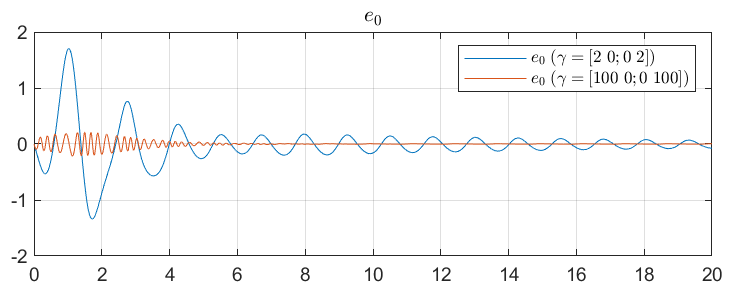
\includegraphics[width=\textwidth]{img/fig08a.png}
        \caption{Erro de Rastreamento}
    \end{subfigure}
    \begin{subfigure}[b]{0.3\textwidth}
        \centering
        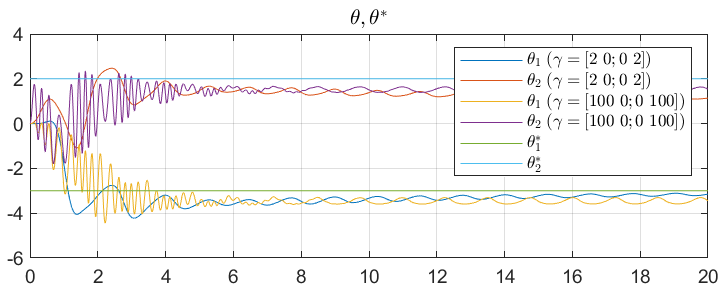
\includegraphics[width=\textwidth]{img/fig08b.png}
        \caption{Ganho de Adaptação}
    \end{subfigure}

    \begin{subfigure}[b]{0.3\textwidth}
        \centering
        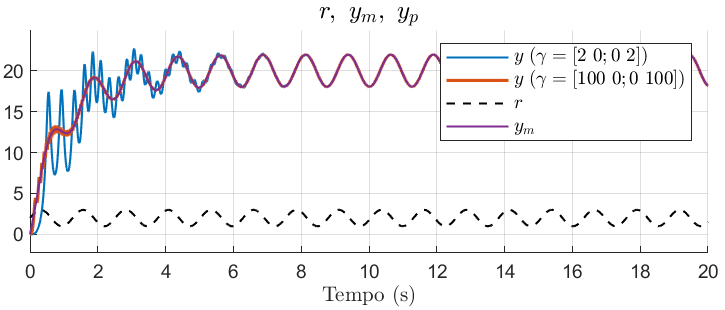
\includegraphics[width=\textwidth]{img/fig08c.png}
        \caption{Resposta do Sistema}
    \end{subfigure}
    \begin{subfigure}[b]{0.3\textwidth}
        \centering
        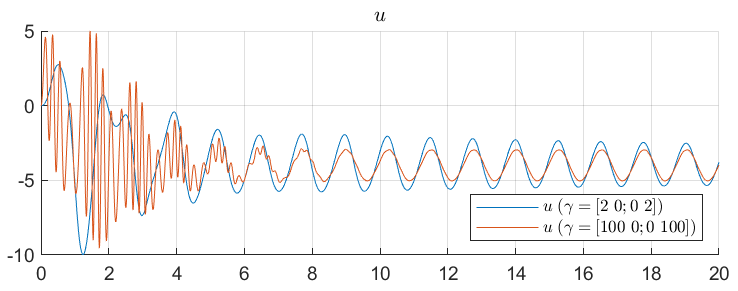
\includegraphics[width=\textwidth]{img/fig08e.png}
        \caption{Sinal de Controle}
    \end{subfigure}

    \begin{subfigure}[b]{0.3\textwidth}
        \centering
        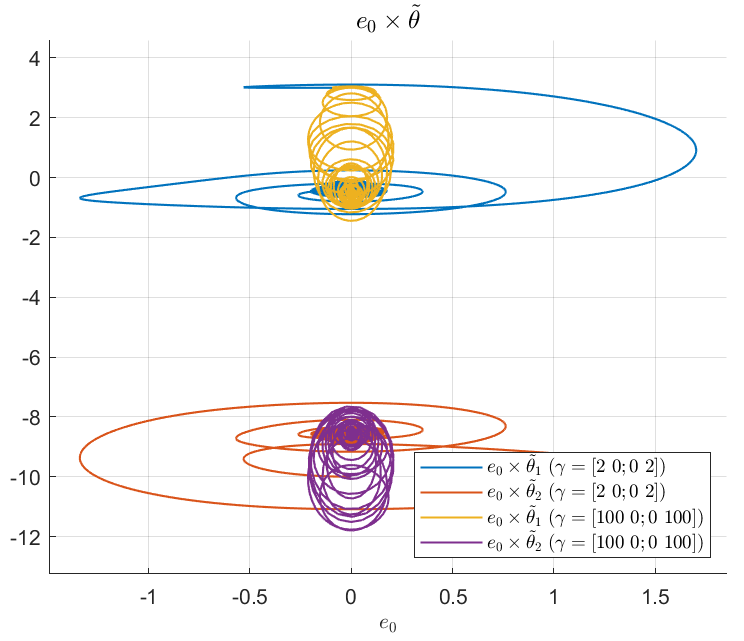
\includegraphics[width=\textwidth]{img/fig08d.png}
        \caption{Diagrama $e_0 \times \tilde{\theta}$}
    \end{subfigure}

    \caption{Resultado da simulação (Script: \textit{simu08.m})}
    \label{fig:sim8}
\end{figure}

\subsubsection{Comentários:}

Nesta simulação, o modelo de referência mantém-se em $M(s) = \frac{10}{s+1}$, com constante de tempo 1 e ganho estático 10, porém o sinal de referência agora inclui um componente senoidal além do degrau: $DC = 2$, amplitude senoidal $A_s = 1$ e frequência $\omega_s = 5$ rad/s. Essa configuração permite avaliar a capacidade do controlador em seguir sinais compostos e dinâmicos. Os principais pontos observados são:

\begin{itemize}
    \item \textbf{Erro de rastreamento ($e_0$):} Na Figura~\ref{fig:sim8}(a), o erro apresenta oscilações permanentes devido à componente senoidal da referência. Com $\Gamma_2 = 100I$, o erro tem amplitude menor e convergência mais rápida no valor médio, enquanto para $\Gamma_1 = 2I$ as oscilações são maiores e a convergência mais lenta.

    \item \textbf{Ganho de adaptação ($\theta$):} Conforme Figura~\ref{fig:sim8}(b), os parâmetros adaptativos não convergem exatamente para os valores ótimos $\theta^* = [-3; 10]$ em ambos os casos, devido à natureza do sinal de referência. O ganho maior ($\Gamma_2$) proporciona convergência mais rápida, porém com maior oscilação transitória.

    \item \textbf{Resposta do sistema:} Na Figura~\ref{fig:sim8}(c), a saída do sistema segue adequadamente o sinal de referência composto, com melhor desempenho em amplitude e fase para $\Gamma_2 = 100I$. Para $\Gamma_1 = 2I$, observa-se atraso maior e amplitude reduzida nas oscilações.

    \item \textbf{Sinal de controle ($u$):} Conforme Figura~\ref{fig:sim8}(d), o controle com $\Gamma_1 = 2I$ apresenta picos maiores e maior esforço durante o transiente, enquanto para $\Gamma_2 = 100I$ o controle é mais suave e estabiliza mais rapidamente.

    \item \textbf{Diagrama de fase ($e_0 \times \tilde{\theta}$):} Na Figura~\ref{fig:sim8}(e), as trajetórias não convergem para a origem, refletindo a presença das oscilações permanentes. A configuração com $\Gamma_1 = 2I$ mostra maior proximidade da origem em relação a $\Gamma_2 = 100I$, indicando comportamento menos oscilatório.

\end{itemize}

\textbf{Conclusão:} A inclusão do componente senoidal no sinal de referência introduz oscilações permanentes no erro e nos parâmetros adaptativos, impedindo a convergência exata para os valores ótimos. Ganhos maiores aceleram a adaptação e reduzem a amplitude do erro médio, mas aumentam as oscilações transitórias. Ganhos menores resultam em resposta mais conservadora, com maior esforço inicial de controle e menor oscilação, porém com erro médio maior. Em ambos os casos, o controlador é capaz de estabilizar a planta instável $P(s) = \frac{1}{s-2}$ e seguir o modelo de referência com o sinal de entrada composto.

\newpage

\subsection{Simulação \#9}
\subsubsection{Configuração do experimento:}
\begin{itemize}
\item \textbf{Planta:} $P(s) = \dfrac{1}{s - 2}$
\item \textbf{Modelo de referência:} $M(s) = \dfrac{1}{s + 1}$
\item \textbf{Condições iniciais:} $y_p(0)=0$, $y_m(0)=0$
\item \textbf{Sinal de referência:} DC = 1, $A_s=0$, $\omega_s=5$ rad/s
\item \textbf{Ganho de matching ótimo:} $\theta^* = [-(2+1)/1;1/1] = [-3;1]$
\item \textbf{Ganho de adaptação:} 
\[
\Gamma_1 = 2 \begin{bmatrix} 1 & 0.35 \\ -0.35 & 1 \end{bmatrix}, \quad
\Gamma_2 = 100 \begin{bmatrix} 1 & 0.35 \\ -0.35 & 1 \end{bmatrix}
\]
\item \textbf{Condição inicial do parâmetro:} $\theta(0) = [0;0]$
\end{itemize}

\subsubsection{Resultados da simulação:}

\begin{figure}[h!]
    \centering
    \begin{subfigure}[b]{0.25\textwidth}
        \centering
        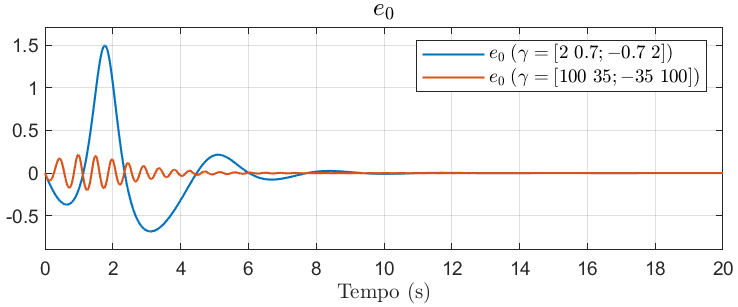
\includegraphics[width=\textwidth]{img/fig09a.png}
        \caption{Erro de Rastreamento}
    \end{subfigure}
    \begin{subfigure}[b]{0.25\textwidth}
        \centering
        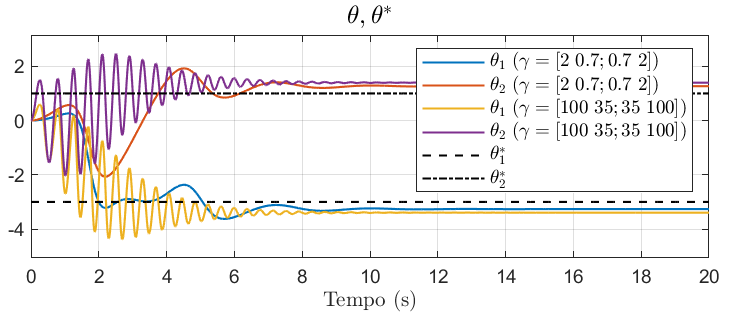
\includegraphics[width=\textwidth]{img/fig09b.png}
        \caption{Ganho de Adaptação}
    \end{subfigure}

    \begin{subfigure}[b]{0.25\textwidth}
        \centering
        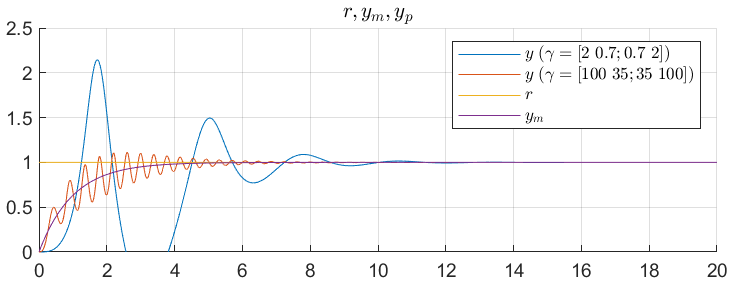
\includegraphics[width=\textwidth]{img/fig09c.png}
        \caption{Resposta do Sistema}
    \end{subfigure}
    \begin{subfigure}[b]{0.25\textwidth}
        \centering
        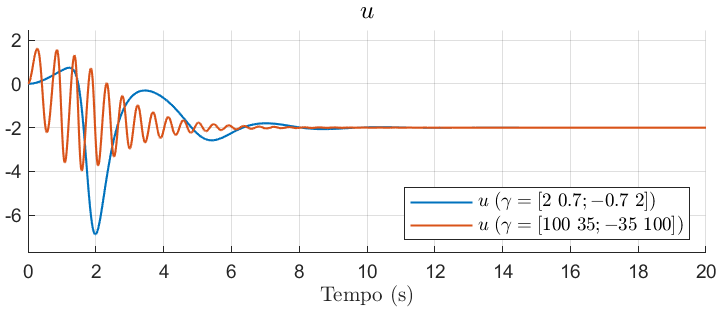
\includegraphics[width=\textwidth]{img/fig09e.png}
        \caption{Sinal de Controle}
    \end{subfigure}

    \begin{subfigure}[b]{0.25\textwidth}
        \centering
        \includegraphics[width=\textwidth]{img/fig09d.png}
        \caption{Diagrama $e_0 \times \tilde{\theta}$}
    \end{subfigure}

    \caption{Resultado da simulação (Script: \textit{simu09.m})}
    \label{fig:sim9}
\end{figure}

\subsubsection{Comentários:}

Nesta simulação, mantêm-se a planta instável $P(s) = \dfrac{1}{s - 2}$ e o sinal de referência puramente constante (DC = 1), mas introduz-se uma modificação importante: os ganhos de adaptação $\Gamma_1$ e $\Gamma_2$ passam a ser matrizes simétricas e não-diagonais, com termos fora da diagonal igual a 0{,}35. Isso permite investigar o impacto de acoplamentos entre os parâmetros adaptativos. Os principais pontos observados são:

\begin{itemize}
    \item \textbf{Erro de rastreamento ($e_0$):} A convergência do erro ocorre de forma estável e eficaz, com desempenho semelhante ao de simulações anteriores com ganho diagonal. A presença de termos fora da diagonal na matriz $\Gamma$ não compromete o rastreamento, indicando robustez do algoritmo adaptativo.

    \item \textbf{Ganho de adaptação ($\theta$):} A trajetória dos parâmetros $\theta$ tende a convergir para valores próximos ao ótimo teórico $\theta^* = [-3;\ 1]$, com dinâmica influenciada pelo acoplamento entre os parâmetros. Observa-se uma interação mais pronunciada entre as componentes de $\theta$, refletida em trajetórias mais entrelaçadas.

    \item \textbf{Resposta do sistema:} A saída da planta acompanha fielmente a resposta do modelo de referência, evidenciando que o sistema adaptativo é capaz de compensar a instabilidade da planta mesmo com uma matriz $\Gamma$ não-diagonal.

    \item \textbf{Sinal de controle ($u$):} O esforço de controle permanece dentro de níveis aceitáveis, com um pico inicial relacionado à correção rápida dos parâmetros. O comportamento do controle é suavizado após o transiente inicial.

    \item \textbf{Diagrama de fase ($e_0 \times \tilde{\theta}$):} O diagrama mostra um padrão de convergência para a origem, com trajetórias mais curvilíneas ou inclinadas do que nas simulações anteriores, evidenciando a influência da matriz $\Gamma$ com acoplamento.

\end{itemize}

\textbf{Conclusão:} A introdução de uma matriz de adaptação não-diagonal mostra-se viável e eficaz para este cenário. O acoplamento entre os parâmetros não prejudica a estabilidade ou o rastreamento, e pode até favorecer uma adaptação mais coordenada, dependendo do caso. Esta simulação demonstra a flexibilidade do esquema adaptativo frente a diferentes configurações matriciais de ganho.

\newpage

\subsection{Simulação \#10}
\subsubsection{Configuração do experimento:}
\begin{itemize}
\item \textbf{Planta:} $P(s) = \dfrac{1}{s - 2}$
\item \textbf{Modelo de referência:} $M(s) = \dfrac{1}{s + 1}$
\item \textbf{Condições iniciais:} $y_p(0)=0$, $y_m(0)=0$
\item \textbf{Sinal de referência:} DC = 2, $A_s=1$, $\omega_s=5$ rad/s
\item \textbf{Ganho de matching ótimo:} $\theta^* = [-(2+1)/1;;1/1] = [-3;;1]$
\item \textbf{Ganho de adaptação:} 
\[
\Gamma_1 = 2 \begin{bmatrix} 1 & 0.35 \\ -0.35 & 1 \end{bmatrix}, \quad
\Gamma_2 = 100 \begin{bmatrix} 1 & 0.35 \\ -0.35 & 1 \end{bmatrix}
\]
\item \textbf{Condição inicial do parâmetro:} $\theta(0) = [0;;0]$
\end{itemize}

\subsubsection{Resultados da simulação:}

\begin{figure}[h!]
    \centering
    \begin{subfigure}[b]{0.25\textwidth}
        \centering
        \includegraphics[width=\textwidth]{img/fig10a.png}
        \caption{Erro de Rastreamento}
    \end{subfigure}
    \begin{subfigure}[b]{0.25\textwidth}
        \centering
        \includegraphics[width=\textwidth]{img/fig10b.png}
        \caption{Ganho de Adaptação}
    \end{subfigure}

    \begin{subfigure}[b]{0.25\textwidth}
        \centering
        \includegraphics[width=\textwidth]{img/fig10c.png}
        \caption{Resposta do Sistema}
    \end{subfigure}
    \begin{subfigure}[b]{0.25\textwidth}
        \centering
        \includegraphics[width=\textwidth]{img/fig10e.png}
        \caption{Sinal de Controle}
    \end{subfigure}

    \begin{subfigure}[b]{0.25\textwidth}
        \centering
        \includegraphics[width=\textwidth]{img/fig10d.png}
        \caption{Diagrama $e_0 \times \tilde{\theta}$}
    \end{subfigure}

    \caption{Resultado da simulação (Script: \textit{simu10.m})}
    \label{fig:sim10}
\end{figure}

\subsubsection{Comentários:}

Nesta simulação, a planta instável e o modelo de referência permanecem inalterados em relação à Simulação \#9. A principal modificação está no sinal de referência, que agora possui uma componente oscilatória (senoide) além do valor DC, tornando o rastreamento mais desafiador. A estrutura de adaptação com matrizes de ganho não-diagonais é mantida.

\begin{itemize}
    \item \textbf{Erro de rastreamento ($e_0$):} O erro apresenta oscilações coerentes com a natureza senoidal do sinal de referência, mas com amplitude limitada, indicando que o sistema consegue acompanhar a referência com boa fidelidade, apesar da maior exigência dinâmica.

    \item \textbf{Ganho de adaptação ($\theta$):} A trajetória dos parâmetros adaptativos mantém estabilidade, com convergência gradual para a vizinhança dos valores ótimos. A oscilação na referência se reflete em oscilações nos parâmetros, especialmente durante os primeiros instantes.

    \item \textbf{Resposta do sistema:} A planta segue o modelo de referência com boa precisão, reproduzindo tanto o valor DC quanto a componente oscilatória da entrada. A performance confirma a eficácia da estrutura adaptativa mesmo sob sinal de referência variado.

    \item \textbf{Sinal de controle ($u$):} O controle exibe oscilações em frequência compatível com a senoide de entrada, mas com amplitude controlada. O esforço de controle aumenta levemente em relação à simulação anterior, como esperado em situações com maior exigência dinâmica.

    \item \textbf{Diagrama de fase ($e_0 \times \tilde{\theta}$):} As trajetórias não convergem diretamente à origem devido à natureza persistente do erro oscilatório. No entanto, o padrão cíclico observado é compatível com um regime permanente de rastreamento senoidal.

\end{itemize}

\textbf{Conclusão:} A Simulação \#10 demonstra a robustez da estrutura adaptativa frente a sinais de referência mais complexos, com bom rastreamento, estabilidade dos parâmetros e controle efetivo. A combinação de matriz $\Gamma$ não-diagonal e entrada mista revela a capacidade do sistema de lidar com variações dinâmicas sem comprometer a convergência e o desempenho.

\newpage

\appendix
\section{Decomposição de Matrizes: Parte Simétrica e Antissimétrica}

Uma matriz $\Gamma$ pode ser decomposta como a soma de uma parte simétrica $\Gamma_s$ e uma parte antissimétrica $A_{as}$:

\begin{equation}
    \Gamma = \Gamma_s + A_{as}
\end{equation}

Considerando uma matriz simétrica da forma:
\begin{equation}
    \Gamma_s = 
    \begin{bmatrix}
        b & 0 \\
        0 & b
    \end{bmatrix}, \quad a, b \in \mathbb{R}^+
\end{equation}

Seja um vetor linha $\mathbf{v} = [x \quad y]$, com $x, y \in \mathbb{R}$, temos:

\begin{equation}
    \mathbf{v} \cdot \Gamma \cdot \mathbf{v}^T > 0
\end{equation}

Expandindo:
\begin{equation}
    \mathbf{v} \cdot \Gamma \cdot \mathbf{v}^T = 
    \mathbf{v} \cdot \Gamma_s \cdot \mathbf{v}^T + 
    \mathbf{v} \cdot A_{as} \cdot \mathbf{v}^T
\end{equation}

Vamos agora considerar uma matriz antissimétrica:
\begin{equation}
    A_{as} = 
    \begin{bmatrix}
        0 & a \\
        -a & 0
    \end{bmatrix}
\end{equation}

Multiplicando:
\begin{align}
    \mathbf{v} \cdot A_{as} \cdot \mathbf{v}^T &= 
    \begin{bmatrix}
        x & y
    \end{bmatrix}
    \begin{bmatrix}
        0 & a \\
        -a & 0
    \end{bmatrix}
    \begin{bmatrix}
        x \\
        y
    \end{bmatrix} \\
    &= a \cdot 
    \begin{bmatrix}
        -y & x
    \end{bmatrix}
    \begin{bmatrix}
        x \\
        y
    \end{bmatrix} \\
    &= a \cdot (-yx + xy) = 0
\end{align}

Portanto, a contribuição da parte antissimétrica na forma quadrática $\mathbf{v} \cdot \Gamma \cdot \mathbf{v}^T$ é nula, ou seja:
\begin{equation}
    \mathbf{v} \cdot A_{as} \cdot \mathbf{v}^T = 0
\end{equation}

Conclui-se que a parte simétrica da matriz $\Gamma$ é a única que contribui para a positividade da forma quadrática.

\end{document}
